\chaptertitle{Mesure de la topologie physique}
\label{chap:udpping}
\introformatting

\lettrine{L}{a} topologie physique d'Internet correspond peut-être davantage à
l'intuition qu'on se fait du réseau lorsque l'on n'est pas familier du protocole
\ip. Elle représente la capacité physique des entités connectées à échanger des
informations. Cette capacité physique est ensuite exploitée au niveau logique,
et les deux topologies sont intrinsèquement reliées, mais la topologie logique
abstrait totalement l'existence d'entités capables de manipuler des paquets sans
être capable d'en émettre ou d'en recevoir par elles-mêmes, ainsi que le détail
des interfaces physiques mobilisées par des entités logiques. Si on peut assez
directement déduire une topologique logique d'une topologie physique, la
réciproque est fausse. Ceci est d'autant plus important que la configuration
physique d'un hôte logique peut avoir un grand impact sur sa performance. Dans
le cas d'un routeur, par exemple, son efficacité dépend souvent grandement de la
performance individuelle de ses interfaces physiques, et non pas uniquement de
la performance de sa couche logique.

La topologie physique a historiquement suscité moins d'attention que la
topologie logique, principalement car les approches historiques reposent sur
l'exploitation de \traceroute qui opère au niveau logique. Pourtant, nos travaux
préliminaires ont mis en évidence les limites d'une approche au niveau logique.
À l'inverse, nos travaux pour tenter de dépasser ces limites, et en particulier
sur l'anti-aliasing, nous ont mis sur la voie d'une approche différente. Au lieu
de corriger l'approche logique en mobilisant des caractéristiques de la
topologie physique, nous avons décidé d'adapter notre méthode pour qu'elle opère
directement au niveau physique. En plus d'éviter beaucoup des problèmes liés à
l'approche logique, elle permet de réaliser une observation d'un objet plus
précis.

Nous présentons ici notre méthode de mesure de la topologique physique. Elle
repose sur une primitive de mesure de bas niveau \udpping inspirée des méthodes
d'anti-aliasing qui sonde une cible depuis un moniteur
(\refsec{udpping-one-to-one}). Cette primitive de mesure de bas niveau est
mobilisée de manière distribuée (depuis un ensemble de moniteurs vers une cible)
pour constituer une primitive de haut niveau (\refsec{udpping-one-to-many}),
pour évaluer le degré au niveau physique d'une cible. Grâce à une méthode
d'échantillonage sans biais nous en déduisons une évaluation de la distribution
de degré physique des routeurs du c\oe{}ur (\refsec{udpping-many-to-many}). Le
principe est validé par de nouvelles simulations (\refsec{udpping-simuls}).
La qualité de cette estimation repose sur des caractéristiques de l'ensemble de
moniteurs utilisé, dont nous avons approfondi l'étude
(\refsec{udpping-monitors}). Nous avons attesté de la faisabilité expérimentale
de notre méthode en réalisant une nouvelle mesure réelle
(\refsec{udpping-measurement}). Avec les retours de cette expérimentation, nous
avons pu établir un protocole complet (\refsec{udpping-protocol}), et effectuer
une validation, à la fois de nos heuristiques d'évaluation de la qualité d'un
ensemble de moniteurs, et réinjecter les résultats dans notre modèle de
simulations pour attester de leur pertinence (\refsec{udpping-validation}). À
l'aide de ces résultats, nous avons pu établir les points forts et les limites
de notre approche et conclure (\refsec{udpping-conclusion}).

\section{Primitive de mesure de bas niveau basée sur \udpping}
\label{sec:udpping-one-to-one}

Un hôte du réseau est un n\oe{}ud appartenant à la fois à \LLL et \LL, qui est
capable de recevoir et de fabriquer des nouveaux paquets. Un hôte se distingue
des autres n\oe{}uds (non-hôtes, tels que les switchs) de \LLL et \LL par son
comportement quand il reçoit un paquet \ip\rfc{791}. Si l'en-tête {\em
Destination Address} appartient à la liste des adresses que cet hôte identifie
comme les siennes, alors il remonte ce paquet à la couche d'abstraction
supérieure. Sinon, il examine l'en-tête {\em Time-to-Live} (ou \ttl) du paquet.
Si sa valeur est zéro, l'hôte émet un nouveau paquet \icmp~{\em Time Exceeded}
en direction de l'adresse indiquée dans l'en-tête {\em Source Address}. Si sa
valeur est supérieure à zéro, l'hôte émet un nouveau paquet \ip avec le même
contenu que le paquet initial, mais dont l'en-tête \ttl est décrémentée de 1 (et
l'en-tête {\em Checksum} mise à jour).

% Dans les deux cas, lorsque l'hôte émet un paquet, il doit choisir sur laquelle
% de ses interfaces il va émettre ce paquet. Ce choix appartient à la couche \LLL,
% et l'interface choisie est identifiée au niveau logique par une adresse \ip, à
% laquelle est associée un identifiant physique dépendant de
% l'implémentation\footnote{Beaucoup d'implémentations reposent sur la convention
% IEEE 802\cite{ieee802}, et les interfaces physiques sont alors identifiées par
% une adresse \mac\rfc{5342}.}. Le nouveau paquet \ip contient alors l'adresse \ip
% correspondante dans son en-tête {\em Source Address}.
% 
% \realfig{udpping-encapsulation.png}{En-têtes des paquets encapsulés} {Un hôte
% source $\overline{u}$ utilise son interface $u$ pour émettre un paquet \udp à destination d'une adresse $v$
% avec un port source $p_u$ et un port destination $p_v$ (en haut).
% L'hôte qui possède l'adresse $v$, $\overline{v}$, émet en réponse un nouveau
% paquet \udp à destination de $u$, mais pour ce faire elle utilise une autre
% interface, $v'$.
% Elle se content d'inscrire le port $p_u$ dans l'en-tête \udp pour que cette
% réponse soit reconnue par la cible (en bas).}{encapsulation}
% 
% Notons que le choix de l'interface de sortie ne dépend pas, \apriori, du paquet
% de couche supérieure (par exemple, \icmp, \tcp ou \udp) que ce paquet \ip
% encapsule. Soit par exemple un paquet \udp envoyé depuis une interface $u$ d'un
% hôte source $\overline{u}$ vers une adresse de destination $v$ d'un hôte
% $\overline{v}$ à destination d'un port $p$.
% L'hôte auquel appartient $v$ peut très bien répondre en utilisant une interface
% $v'$ qui lui appartient également, et inscrire $v'$ dans la {\em Source Address}
% du paquet \ip encapsulant la réponse, ainsi que $p_u$ dans l'en-tête {\em
% Destination Port} du paquet \udp.
% C'est le port $p_u$ qui sera utilisé par $\overline{u}$ pour reconnaître cette
% réponse, et non l'adresse $v'$ inscrite dans le paquet \ip
% (\reffig{encapsulation}). On définit donc :
% 
% \begin{definition}[Voisins d'un hôte associés à une interface] Soit
% $\overline{u}$ un hôte de \LLL. Pour chaque $u' \in \overline{u}$, on note
% $V(\overline{u}, u')$ et on appelle {\em ensemble des voisins de $\overline{u}$
% associés à l'interface $u'$} l'ensemble des adresses \ip $v \in \IPSet$ de
% $\overline{u}$ tels que $(u, v)$ est le support physique d'un lien
% $(\overline{u}, \overline{v})$ (et en particulier, $\overline{v}$ est un voisin
% de $\overline{u}$ dans \LLL). On note $\overline{V}(\overline{u}, v)$ l'ensemble
% des hôtes sous-jacents à ces adresses.
% \end{definition}
% 
% Et, de manière analogue :
% 
% \begin{definition}[Destinations d'un hôte associées à une interface]
% Soit $\overline{u}$ un hôte de \LLL. Pour chaque $u' \in \overline{u}$ on note
% $D(\overline{u}, u')$ et on appelle {\em ensemble des destinations
% associées à $u'$} l'ensemble des adresses \ip $v \in \IPSet$ de \LLL telles que
% $u'$ est choisie par $\overline{u}$ pour émettre un paquet \ip à destination de
% $v$. On note $\overline{D}(\overline{u}, u')$ l'ensemble des hôtes sous-jacents
% à ces adresses.
% \end{definition}
% 
% Remarquons que la plupart du temps, si la politique de routage locale est
% correctement implémentée, alors pour un hôte source $\overline{u}$, un voisin
% $\overline{v}$ de $\overline{u}$ via un lien $(u, v)$, et un hôte destination
% $\overline{w}$ désigné par une adresse $w$ telle que $w \in D(\overline{u}, v)$
% (c'est à dire tels que $\overline{u}$ choisit l'interface $v$ le reliant à
% $\overline{v}$ pour envoyer des paquets vers $w$), alors $D(\overline{v},
% \overline{w}) \leq D(\overline{u}, \overline{w})$. En règle générale, si le
% routage s'effectue sans cycle, il existe un chemin sans cycle $\overline{u}
% \rightarrow \overline{v} \rightarrow \ldots \rightarrow \overline{w}$ (qui en
% particulier ne repasse pas par $\overline{u}$).

Soit $\overline{m}$ un hôte que l'on appelle un {\em moniteur} muni d'une unique
interface désignée par son adresse \ip $m$, depuis lequel nous sommes capable
d'exécuter un programme avec un accès privilégié. Soit $\overline{t}$ un hôte
que l'on appelle une {\em cible} et dont on connaît l'une des adresses \ip $t$.
Supposons que l'on envoie un paquet \udp depuis $\overline{m}$ vers $t$,
contenant un message arbitraire, et à destination d'un port non utilisé $p$.
Lorsque $\overline{t}$ réceptionne ce paquet, sa couche \LLL reconnaît le paquet
comme lui étant destiné et le transmet à la couche supérieure --- en
l'occurence, \udp.
À ce niveau, l'hôte identifie que le paquet est à destination d'un port non
utilisé, et émet un paquet \icmp {\em Destination Unreachable (Code 3/Port
Unreachable)} dont la destination est $m$\cite{rfc1122,rfc1123}. Le paquet \icmp
émis est encapsulé dans un paquet \ip, dont l'en-tête {\em Source Address} est
en principe l'interface d'adresse \ip $i$ choisie par l'hôte pour envoyer un
paquet à destination de $m$. Notons en particulier que cette interface $i$ {\em
peut} être différente de $t$, bien qu'elle appartienne également à l'ensemble
$\overline{t}$ des interfaces de la cible (\reffig{encapsulation-udpping}).
Cette technique est inspirée de la technique d'{\em anti-aliasing} utilisée par
exemple par \iffinder~\cite{keysiffinder,iffinder,280555,GovindanT00}.

\realfig{udpping-encapsulation-udpping.png}{En-têtes des paquets \udpping} {Un
hôte moniteur $\overline{m}$ utilise son unique interface $m$ pour émettre un paquet \udp avec un port source
quelconque $p_m$ et un port destination arbitraire non utilisé $p_t$ vers
l'adresse \ip $t$ (en haut). À la réception, l'hôte cible $\overline{t}$ qui
possède l'adresse \ip $t$ reconnaît un port non utilisé et émet un paquet \icmp
d'erreur en direction de $m$. Pour ce faire, elle utilise une certaine interface
$i = m(t)$.} {encapsulation-udpping}

Nous nommons \udpping l'outil qui permet d'envoyer des paquets \udp vers un port
non utilisé d'une adresse cible $t$ et de réceptionner les paquets d'erreur
\icmp et de reconnaître les réponses $i$. Il peut être exécuté depuis
n'importe quel hôte avec des privilèges permettant d'envoyer des paquets \udp et
de réceptionner les paquets \icmp (ce dernier privilège étant un privilège {\em
root} sur la plupart des systèmes). Dans ce chapitre, nous utiliserions ainsi la
notation suivante :

\begin{definition}[Observation d'une cible depuis un moniteur] Soit $i$ le
résultat de \udpping depuis $m$ vers $t$. Si ce résultat est une adresse (c'est
à dire qu'une réponse a été obtenue après l'envoi de la sonde), on note $m(t) =
i$ et on l'appelle {\em observation de $t$ depuis $m$}.
\label{def:udpping-one-to-one}
\end{definition}

Par construction, $m(t) \in \overline{t}$, et plus précisément, $m(t)$ est
l'{\em interface choisie par l'hôte $\overline{t}$ pour émettre à destination de
$m$}. Ainsi, $m(t)$ dépend de $m$ (d'où cette notation).
Si $\overline{t}$ est un routeur, en particulier, alors $m(t)$ sera choisie en
fonction de la politique de routage de $\overline{t}$. Par exemple, $m(t)$
pourrait être l'interface de $\overline{t}$ qui la relie au niveau {\em
physique} au prochain {\em hop} dans le plus court chemin au niveau {\em
logique} depuis $\overline{t}$ vers $\overline{m}$
(\reffig{udpping-one-to-one-example}).

\realfig{udpping-one-to-one-example.png}{Choix de l'interface $m(t)$ par la
cible $\overline{t}$} {Un moniteur $m$ envoie une sonde \udpping vers $t$. La
cible $\overline{t}$ répond en utilisant une interface $m(t)$ qui se trouve être
différente de $t$, et qui correspond à ici à l'interface vers le premier {\em
hop} du plus court chemin de retour vers $m$.} {udpping-one-to-one-example}

Remarquons que contrairement à notre primitive de mesure basée sur \traceroute
(\ref{sec:traceroute-one-to-one}), la qualité de la réponse est binaire: soit le
moniteur reçoit une réponse de la cible, et on note cette réponse $m(t)$, soit
le moniteur ne reçoit pas de réponse (si la sonde n'a pas atteint
la cible, ou que la cible n'a pas répondu, ou que la réponse n'a pas atteint le
moniteur). En particulier, l'ensemble $\mathbb{M}(\overline{t}) = \cup_{t' \in
\overline{t}} {\mathbb M}(t)$ des moniteurs observant une cible est exactement
l'ensemble des moniteurs ayant obtenu une réponse à leur sonde.

Pour une interface $t \in \overline{t}$ donnée d'une cible donnée, on considère
l'ensemble des hôtes tels que, si on exécutait \udpping depuis cet hôte vers
$\overline{t}$, on obtiendrait $t$.

\begin{definition}[N\oe{}uds capables d'observer une interface donnée d'une
cible] Soit $\overline{t}$ une cible et $t' \in \overline{t}$ une interface de
cette cible (égale ou non à $t$). On note ${\mathbb M}(t')$ l'ensemble $\{ m,
m(t) = t'\}$ et on l'appelle {\em ensemble des n\oe{}uds capables d'observer
l'interface $t'$}.
\end{definition}

Un certain type d'interfaces est particulièrement difficile à observer. Soit une
cible $\overline{t}$ munie d'une certaine interface $t'$ telle que $t'$ relie
$\overline{t}$ à un ensemble de n\oe{}uds qui sont tous dans le bord. Alors pour
observer $t'$ en utilisant des sondes \udp, il faut nécessairement disposer d'un
moniteur qui est précisément dans cet ensemble; en particulier, un tel moniteur
est nécessairement dans le bord.

On définit donc :

\begin{definition}[Interface tournée vers le bord (resp. vers le c\oe{}ur)] Soit
$t' \in \overline{t}$ une interface telle que $t'$ est présente sur tous les
chemins entre n'importe quel noeud de $\mathbb(t')$ et le c\oe{}ur. On dit alors
que $t'$ est {\em tournée vers le bord}. Inversement, si $t'$ n'est pas {\em
tournée vers le bord}, on dit qu'elle est {\em tournée vers le c\oe{}ur}, et
dans ce cas il existe au moins un moniteur dans le c\oe{}ur capable d'observer
$t'$.
\end{definition}

% Nous allons distinguer un certain type d'interfaces qui sont particulièrement
% difficiles à observer. Soit une interface $t'$ d'une cible $\overline{t}$ telle
% que tous les n\oe{}uds de $\overline{v} \in \overline{V}(\overline{t}, t')$ sont
% dans le bord.
% Alors chaque $\overline{v}$ est racine d'un arbre \LLL que l'on note
% $A(\overline{v})$.
% Si le routage s'effectue sans cycle, alors $D(\overline{t}, t') =
% \cup_{\overline{v} \in \overline{V}(\overline{t}, t')} A(v)$. Or, les n\oe{}uds de
% ${\mathbb M}(t')$ recoivent des sondes retour de \udpping, donc on peut déduire
% que le routage s'effectue sans cycle; on peut en déduire que ${\mathbb M}(t')
% \subset D(\overline{t}, t') = \cup_{\overline{v}} A(\overline{v})$. En
% particulier, chaque n\oe{}ud $m \in {\mathbb M}(t')$ est un n\oe{}ud du bord, ce qui
% justifie la définition suivante :
% 
% \begin{definition}[Interface tournée vers le bord ou vers le c\oe{}ur] Soit $t' \in
% \overline{t}$ une interface telle que tous les n\oe{}uds de
% $\overline{V}(\overline{t}, t')$ soient dans le bord. Alors tous les n\oe{}uds de
% ${\mathbb M}(t')$ sont également dans le bord, et on dit que $t'$ est une {\em
% interface tournée vers le bord} de $\overline{t}$. Sinon, on dit que $t'$ est
% une {\em interface tournée vers le c\oe{}ur}.
% \end{definition}

Autrement dit, si $t'$ est une interface tournée de $\overline{t}$ vers le bord,
alors un moniteur $m$ ne peut observer $t'$ avec \udpping que si $m$ dans
l'arbre relié au c\oe{}ur en passant par $t'$.

Cette section nous a permis de définir et d'interpréter la primitive de mesure
$m \in {\mathbb M}(\overline{t}) \mapsto m(t) \in \IPSet$. Pour la suite, nous
appelerons cette primitive notre {\em primitive de mesure de bas niveau basée
sur \udpping}.

\section{Primitive de mesure de haut niveau basée sur \udpping} 
\label{sec:udpping-one-to-many}

Nous avons vu que \udpping permet d'obtenir, depuis un moniteur $m$, une
interface d'une cible $\overline{t}$ désignée par l'une de ses adresses \ip $t$,
et que cette interface $m(t)$ dépend du moniteur $m$. Des sondes \udp de cette
nature ont déjà été utilisées pour résoudre le problème de l'{\em anti-aliasing}
: étant données deux adresses $t_1$ et $t_2$ d'une cible, il s'agit de
déterminer si $t_1$ et $t_2$ appartiennent au même hôte, c'est à dire si
$\overline{t_1} = \overline{t_2}$. Si l'on exécute \udpping (ou \iffinder)
depuis un moniteur $m$ vers $t_1$ et $t_2$ et que l'on obtient le même résultat
$t$ (qui peut être ou non égal à $t_1$ ou $t_2$), alors on conclut que $t_1$,
$t_2$ et $t$ sont des {\em alias} d'un même hôte $\overline{t} = \overline{t_1}
= \overline{t_2}$.
Nous nous intéressons ici au problème inverse: étant donnée une cible
$\overline{t}$ désignée par l'une de ses adresses \ip $t$, déterminer la liste
de toutes ses interfaces.

Considérons, comme illustré en \reffig{udpping-two-to-one}, le cas simplifié
d'une cible $\overline{t}$ désignée par une adresse \ip $t$, ayant exactement
deux interfaces $t$ et $t'$, et deux moniteurs $m \in D(\overline{t}, t)$ et $m'
\in M(\overline{t},t')$. Alors $m(t) = t$ et $m'(t) = t'$.
En particulier, puisque chaque interface de $\overline{t}$ est observée par l'un
des deux moniteurs, alors $\{ m(t), m'(t) \} = \overline{t}$. Autrement dit, si
pour chaque interface de $\overline{t}$ on dispose d'un moniteur qui permet
d'observer cette interface, on obtient exactement la liste des interfaces de
$\overline{t}$ (\reffig{udpping-two-to-one}).

\realfig{udpping-two-to-one.png}{Cas simplifié d'une cible à deux interfaces
avec routage basique} {La cible $\overline{t}$ dispose d'exactement deux
interfaces qui sont utilisées chacune pour adresser deux parties disjointes du
réseau. Si l'on dispose d'un moniteur dans chacune de ces parties disjointes,
alors on peut observer les deux interfaces de $\overline{t}$.}
{udpping-two-to-one}

On définit, plus généralement :

\begin{definition}[Interfaces d'une cible observées par un ensemble de
moniteurs]
Soit $M$ un ensemble de moniteurs. On note $M(t)$ et on appelle {\em ensemble
des interfaces observées par $M$ pour la cible $t$} l'ensemble $M(t) = \{
m(t), m \in M \} \subset \overline{t}$.
\end{definition}

L'objectif est alors d'obtenir $M(t) \supset \overline{t}$ pour obtenir
l'égalité. Soit une cible $\overline{t} = \{ t_0, \ldots, t_k \}$ désignée par
une adresse \ip $t$, et un ensemble de moniteurs $M$. Alors si pour chaque $j
\in [\![0, k]\!]$, il existe au moins un certain $m_j \in M$ tel que $m_j \in
{\mathbb M}(\overline{t}, t_j)$, alors $M(t) = \overline{t}$. Autrement dit, si l'ensemble $M$
est correctement réparti par rapport aux interfaces de $\overline{t}$, alors en
exécutant \udpping depuis chacun des moniteurs de $M$, on obtient la liste
complète des interfaces $\overline{t}$.

La difficulté repose donc sur l'obtention d'un ensemble de moniteurs $M$
adéquat, capable d'observer toutes les interfaces d'une cible. Cependant, cette
approche se révèle peu exploitable en pratique dans le cas d'une cible
quelconque, à cause des interfaces tournées vers le bord. En effet, nous avons
vu précédemment que pour être capable d'observer une interface tournée vers le
bord avec \udpping, il faut disposer d'un moniteur qui se trouve précisément
dans un arbre du bord qui est relié au c\oe{}ur par cette interface. Si nous
souhaitons réaliser cette condition pour n'importe quelle cible, il faudrait
avoir un ensemble de moniteurs dans chaque sous-arbre du bord, c'est à dire tous
les n\oe{}uds du bord\ldots

On va donc s'intéresser uniquement aux interfaces dans le c\oe{}ur d'une cible. Si
$\overline{t}$ est dans le bord, alors elle ne possède qu'une seule interface
dans le c\oe{}ur. Inversement, si une cible est dans le c\oe{}ur, alors elle
possède au moins deux interfaces dans le c\oe{}ur (\reffig{udpping-core}). Il existe un cas
particulier notable, où un n\oe{}ud du c\oe{}ur possède au moins une interface dans le
bord. On appelle ce type de n\oe{}uds un n\oe{}ud de {\em branchement}, et tout arbre
du bord est relié au c\oe{}ur par un unique n\oe{}ud de branchement. Cette notion sera
mobilisée pour identifier certaines configurations
(\refsec{udpping-monitors}).

Dans le cas où nous nous intéressons à des routeurs dans le c\oe{}ur, nous
pouvons espérer que si nous disposons d'un ensemble suffisamment grand et bien
réparti de moniteurs, alors nous pouvons bien observer toutes ses interfaces
dans le c\oe{}ur. En effet, si des interfaces ne sont pas observées par un tel
ensemble, c'est que ces interfaces ne sont probablemment pas sollicitées dans le
fonctionnement normal du routeur, et peuvent être négligées du point de vue de
la topologie. L'hypothèse selon laquelle un ensemble de moniteurs de taille
raisonnable suffit à observer toutes les interfaces dans le c\oe{}ur d'une cible
donnée est validée plus précisément à l'aide de simulations
(\refsec{udpping-simuls}).

\begin{figure}[!ht]\centering
\subfloat{\includegraphics[width=0.9\columnwidth]{images/udpping-core1.png}}
\\
\subfloat{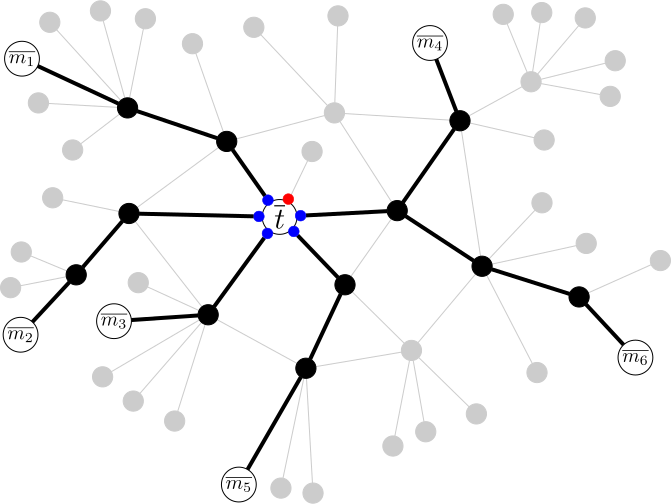
\includegraphics[width=0.9\columnwidth]{images/udpping-core2.png}}
\caption[Cas d'une cible dans le c\oe{}ur et d'une cible dans le bord]{En haut (a):
la cible $\overline{t}$ est dans le bord, et possède une seule interface tournée
vers le c\oe{}ur (en bleu), qu'on observe avec un ensemble de moniteurs bien
réparti. En bas (b): la cible $\overline{t}$ est dans le c\oe{}ur, et on observe
toutes ses interfaces tournées vers le c\oe{}ur (en bleu).}
\label{fig:udpping-core}
\end{figure}
 
Pour une certaine cible $t \in \IPSet$, nous considérons alors $M \subset
{\mathbb M}(t) \mapsto M(t) \subset \IPSet$ notre {\em primitive de mesure de
haut niveau basée sur \udpping}.

\section{Echantillonage rigoureux dans le c\oe{}ur}
\label{sec:udpping-many-to-many}

Nous avons vu que sous réserve de disposer d'un ensemble de moniteurs $M$
suffisamment grand et suffisamment bien réparti, nous étions capables d'obtenir
la liste des interfaces d'une cible $t$ appartenant à un routeur $\overline{t}$
dans le c\oe{}ur. En particulier, $|M(t)| = |\overline{t}|$, le degré physique de 
$\overline{t}$. Si nous étions capables d'obtenir un ensemble de
cibles $T$ uniformément réparties dans le c\oe{}ur, en calculant la distribution
des degrés observés depuis $M$ vers $T$, alors nous obtiendrions une estimation
de la distribution des degrés physiques du c\oe{}ur, et il suffirait d'avoir $|T|$ assez
grand pour garantir la représentativité de cet échantillon.

Malheureusement, nous ne savons pas tirer un ensemble uniformément aléatoire
d'hôtes, et encore moins cibler spécifiquement les routeurs du c\oe{}ur tout en
conservant l'uniformité. En revanche, nous sommes capables de tirer uniformément
un ensemble d'{\em adresses \ip}, qui ne sont autres que des nombres entiers
particuliers.
À partir d'un tel ensemble, nous pouvons réaliser des transformations
(filtrages) qui, chacune, conservent l'uniformité de l'échantillon en ce
qu'elles sont indépendantes du degré des hôtes. Nous pouvons trouver une série
de transformations uniformes qui réduise notre ensemble à un ensemble uniforme
d'adresses \ip d'interfaces dans le c\oe{}ur de routeurs du c\oe{}ur, et qui
répondent correctement aux sondes \udpping
(\refsubsec{udpping-many-to-many-addresses}). Il ne s'agit pas encore d'un
ensemble uniforme de {\em routeurs}, mais d'un ensemble d'{\em adresses}.
Cependant, nous sommes capables de déduire la distribution de degrés des
routeurs du c\oe{}ur à partir de la distribution de degrés de cet échantillon,
par une méthode de correction du biais (\refsubsec{udpping-many-to-many-bias}).

\subsection{Echantillonage d'adresses \ip de routeurs du c\oe{}ur}
\label{subsec:udpping-many-to-many-addresses}

On part initialement d'un ensemble $T_0$ d'entiers de 32 bits choisis
uniformément aléatoirement, et on applique une série de transformations
uniformes $(\varphi_k)$, indépendantes du degré des hôtes sous-jacents, pour
construire des ensembles filtré définis par $T_{n+1} = \varphi_n(T_n) \subset
T_n$.
Chacune des transformations réalisées est indépendante des autres et peut,
théoriquement, être opérée dans n'importe quel ordre. Cependant, pour des
considérations opérationelles, certaines sont plus commodes à exécuter le plus
tôt possible, par exemple parce qu'elles réduisent le nombre de calculs à
effectuer pour les filtrages les plus lourds qu'on réalise ultérieurement.

La première transformation $\varphi_1$ écarte les adresses qui (a) ne
correspondent pas à des adresses \ip routables \rfc{7020} ou qui (b) sont
routables mais pour lesquelles les moniteurs de notre ensemble n'obtiennent pas
de réponses valides. Nous supposons également qu'il n'y a pas de raison
intrinsèque pour que les hôtes de faible degré se comportent différemment des
hôtes de fort degré à ce titre, et donc que cette transformation est
indépendante du degré.

La deuxième transformation $\varphi_2$ vise à éliminer les hôtes qui ne sont pas
des routeurs du c\oe{}ur, c'est à dire les routeurs du bord. Les routeurs du
bord sont situés dans un arbre, et par conséquent, ils n'ont qu'une seule
interface tournée vers le c\oe{}ur. Soit $\overline{t}$ un routeur du bord. Pour
chaque moniteur $m$, il y a trois cas possibles: soit $m$ n'obtient pas de
réponse, soit $m$ est dans le même arbre que $\overline{t}$ et il observe alors
une interface tournée vers le bord de $\overline{t}$, soit $m$ n'est pas dans le
même arbre et il observe l'unique interface de $\overline{t}$ qui est tournée
vers le c\oe{}ur. Nous verrons en~\refsubsec{udpping-monitors-coloc} que nous
sommes capables de caractériser ces cas, c'est à dire détecter si un moniteur se
trouve dans le même arbre qu'une cible (\reffig{udpping-filter-core}, haut).
Réciproquement, si au moins deux interfaces distinctes $t$ et $t'$ sont
observées par des moniteurs qui ne sont pas dans le même arbre que la cible,
alors $\overline{t}$ ne peut être dans le bord (\reffig{udpping-filter-core},
bas).
Pour détecter un hôte qui n'est pas un routeur du c\oe{}ur, il suffit donc
d'écarter les adresses $t$ telles que $M^*(t)$, qui est égal à $M(t)$ privé des
éventuelles interfaces observées par des moniteurs se trouvant dans le même
arbre, soit réduit à 0 (aucune observation) ou 1 interface (l'unique interface
dans le c\oe{}ur de $\overline{t}$). Dans tous les cas, si l'on supprime toutes
les adresses $\overline{t}$ telles que $|M^*(t)| \leq 1$, alors toutes les
adresses restantes appartiennent nécessairement à des routeurs du c\oe{}ur.
Comme cette configuration n'est pas reliée au degré, cette transformation est
également indépendante du degré.

\begin{figure}[!ht]\centering
\subfloat{\includegraphics[width=0.88\columnwidth]{images/udpping-filter-core1.png}}
\\
\subfloat{\includegraphics[width=0.88\columnwidth]{images/udpping-filter-core2.png}}
\caption[Filtrage des adresses de routeurs du c\oe{}ur]{En haut (a): Une cible dans
le bord $\overline{t}$ possède une unique interface tournée vers le c\oe{}ur, $t$, qui est observée par tous les moniteurs
qui ne sont pas dans le même arbre (en haut). En bas (b): Une cible dans le
c\oe{}ur, en revanche, a au moins 2 interfaces observables par des moniteurs qui ne
sont pas dans le même arbre.}
\label{fig:udpping-filter-core}
\end{figure}

% \phfig{Filtrage des cibles à la racine d'arbre du bord contenant au moins un
% moniteur} {Une cible $\overline{t}$ connecte la racine $\overline{r}$ d'un arbre
% du bord dans lequel se trouve un moniteur $\overline{m}$, ce qui conduit à
% l'observation (par le moniteur $\overline{m}$) d'une interface qui n'est pas
% dans le c\oe{}ur. On détecte cette situation et on supprime $\overline{t}$ de
% l'ensemble des cibles.} {udpping-filter-udpping}

La dernière transformation $\varphi_3$ vise à éliminer les adresses qui
correspondent à des interfaces de routeur du c\oe{}ur mais qui ne sont pas
elles-mêmes des interfaces dans le c\oe{}ur. Sous l'hypothèse que $M$ soit
suffisamment grand et suffisamment bien distribué, alors $M(t)$ est exactement
l'ensemble des interfaces de $\overline{t}$ dans le c\oe{}ur. Il suffit donc de
tester si $t \in M(t)$ et supprimer $t$ si $t \notin M(t)$, opération qui est
toujours indépendante du degré de $\overline{t}$.

On note $\varphi = \varphi_3 \circ \varphi_2 \circ \varphi_1$ et $T =
\varphi(T_0)$.

À ce stade, $T$ est un ensemble uniformément aléatoire (par rapport à la
distribution de degrés) d'adresses d'interfaces dans le c\oe{}ur de routeurs du
c\oe{}ur.

\subsection{Correction du biais}
\label{subsec:udpping-many-to-many-bias}

Nous suppons que nous disposons d'un ensemble $T$ uniformément aléatoire
d'adresses d'interfaces dans le c\oe{}ur de routeurs du c\oe{}ur, et nous cherchons à
obtenir une estimation de la distribution des degrés physiques des routeurs du
c\oe{}ur.

Remarquons tout d'abord que nous n'avons pas ici échantillonné des {\em
routeurs} (hôtes), mais des {\em adresses~\ip}. Or, chaque routeur du c\oe{}ur
possède autant de chances d'être sélectionné par adresse qu'il possède
d'adresses, c'est à dire que plus son degré est élevé, plus il a de chances,
proportionellement à son degré (son nombre d'interfaces dans le c\oe{}ur), d'être
tiré par son adresse.
Notons $p_k$ la fraction réelle de routeurs de degrés $k$ dans la distribution
de degrés, et $p'_k$ la fraction des adresses appartenant à des routeurs du
c\oe{}ur de degré $k$. Alors, d'après notre remarque, $p'_k \sim k \cdot
p_k$.
Le facteur linéaire est simplement un facteur de normalisation assurant que
$\sum_k p_k = \sum_k p'_k = 1$, et on obtient donc :
$$ p_k = \frac{p'_k}{k} \cdot \frac {1}{\sum_i \frac{p'_i}{i}} $$

Pour obtenir une estimation de $p_k$ à partir d'un échantillon $T$, il suffit
donc de mesurer $p'_k(T)$, la fraction de routeurs de degré $k$ parmi les
routeurs sous-jacents aux adresses de $T$, et de corriger cette estimation en
utilisant la formule ci-dessus. On obtient finalement :
$$ p_k(T) = \frac {p'_k(T)}{k} \cdot \frac {1}{\sum_i \frac{p_i(T)}{i}} $$

La qualité de l'estimation $ p_k \simeq p_k(T) $ dépend alors uniquement de la
nature de la distribution $(p_k)$ et de $|T|$. Cette transformation de
distribution est illustrée en~\reffig{udpping-bias}.

\begin{figure}[!ht]\centering
\subfloat{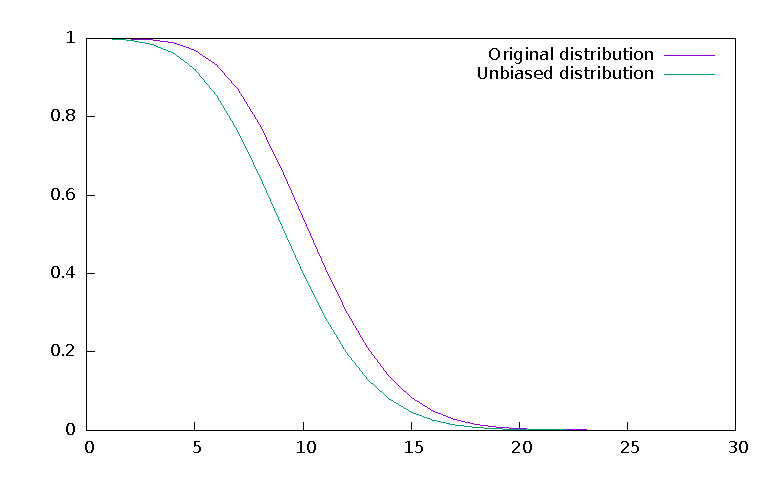
\includegraphics[width=\columnwidth]{images/udpping-unbiasing-poisson.eps}}
\\
\subfloat{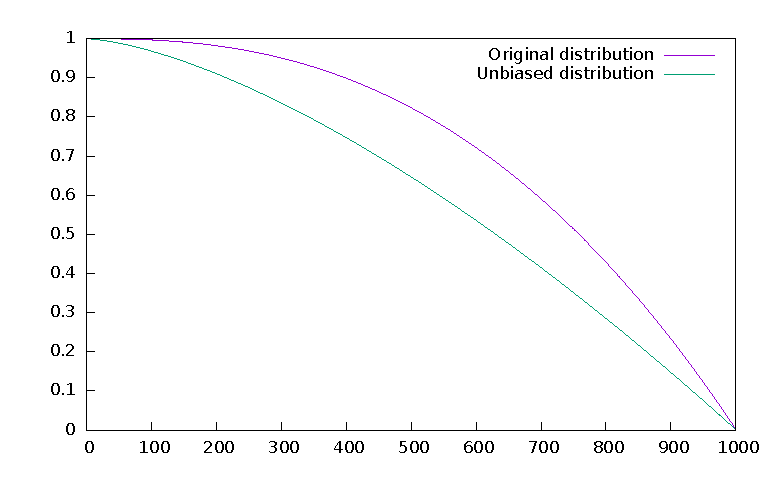
\includegraphics[width=\columnwidth]{images/udpping-unbiasing-powerlaw.eps}}
\caption[Transformation de correction du biais]{Fonction de
distribution cumulative inversée ({\em ICDF})) d'une loi de Poisson
de moyenne $\lambda=10$ (en haut), et d'une loi de puissance d'exposant $\alpha
= 2.5$  (en bas) avant et après la transformation de correction du biais.}
\label{fig:udpping-bias}
\end{figure}

Remarquons que le biais de sélection que nous venons de décrire possède un atout
important. En effet, on s'attend à ce qu'il y ait relativement peu de n\oe{}uds
de degré élevé (ce qui sera confirmé en~\refsec{udpping-measurement}), ce qui
pourrait présenter le risque de ne pas en échantillonner. Si nous
échantillonions les routeurs de manière strictement uniforme, un routeur de
degré $k$ serait échantilloné avec une probabilité $p_k$. Or, notre biais de
sélection nous fait échantilloner un routeur de degré $k$ avec une probabilité
$k \cdot p_k$. Ceci nous permet d'avoir une bonne confiance dans la qualité de
l'estimation à la fois pour les faibles degrés (qui sont très nombreux) et pour
les forts degrés (dont l'échantillonage est assuré par notre méthode).

\section{Validation du principe}
\label{sec:udpping-simuls}

Notre approche repose sur l'hypothèse que nous pouvons disposer d'un ensemble de
moniteurs $M$ suffisamment grand et suffisamment bien réparti pour pouvoir
observer toutes les interfaces dans le c\oe{}ur d'un routeur du c\oe{}ur
quelconque.
La question à laquelle nous voulons répondre est la suivante : quel est le
risque que notre estimation du degré d'un n\oe{}ud soit différente de son degré
réel, et de combien de moniteur devons nous disposer pour obtenir une estimation
fiable de la distribution de degrés ?

Pour répondre à cette question, nous avons entrepris une démarche de simulations
sur des graphes synthétiques. Nous avons utilisé comme moniteurs des n\oe{}uds de
degré 1 (représentant des hôtes terminaux). Les cibles étaient tous les n\oe{}uds
du c\oe{}ur, afin de découpler la problématique qui nous intéresse de la
problématique d'échantillonage qui est un problème purement statistique et qui
n'est pas directement lié à notre méthode. Nous avons supposé que chaque cible
répondait à un moniteur en empruntant le plus court chemin (ou l'un des plus
courts chemins choisi aléatoirement en cas de choix multiples). Nous nous sommes
intéressés à deux modèles de topologies : les topologies en loi de Poisson,
typiques des distributions de degrés homogènes, et les topologies en loi de
puissance, typiques des distributions de degrés hétérogènes. Nous ne nous
attendons pas à ce que la distribution réelle d'Internet corresponde
exactement à l'un de ces deux modèles, mais ils représentent des cas extrêmes de ce qu'elle pourrait
être. Nous avons simulé l'observation de la distribution de degrés pour
différentes tailles de l'ensemble des moniteurs : $12$, $25$, $50$, $100$,
$200$, $400$ et $800$ moniteurs.

Le résultat de ces simulations est exposé
en~\reffig{udpping-simuls-poisson-detail}
et~\reffig{udpping-simuls-powerlaw-detail}.
Comme on peut s'y attendre, la distribution de degrés est assez mal observée
dans le cas de $12$ moniteurs. En particulier, le degré maximum observé est celui du
nombre total de moniteurs, $12$, et les n\oe{}uds de fort degré ont leur degré très
sous-évalué. Cependant, on peut relever que même avec $12$ moniteurs, la nature
de la distribution (homogène ou hétérogène) apparaît très clairement. Lorsqu'on
augmente le nombre de moniteurs, la qualité de l'observation s'accroît
rapidement. Dès $200$ moniteurs, la distribution réelle est indiscernable de la
distribution observée dans le cas homogène. Dans le cas hétérogène,
l'observation est très fidèle jusqu'à un très haut degré, au delà duquel la qualité de
l'estimation s'appauvrit. Ceci n'est pas surprenant, dans la mesure où le degré
mesuré ne peut excéder le nombre total de moniteurs, et où les chances de
manquer certaines interfaces grandit lorsque le degré croît vers ce nombre.
Toutefois, pour les n\oe{}uds de degré relativement faible, par exemple inférieur à
$20$, la distribution observée est indiscernable de la distribution réelle.


% \begin{figure}[!ht]\centering
% \subfloat{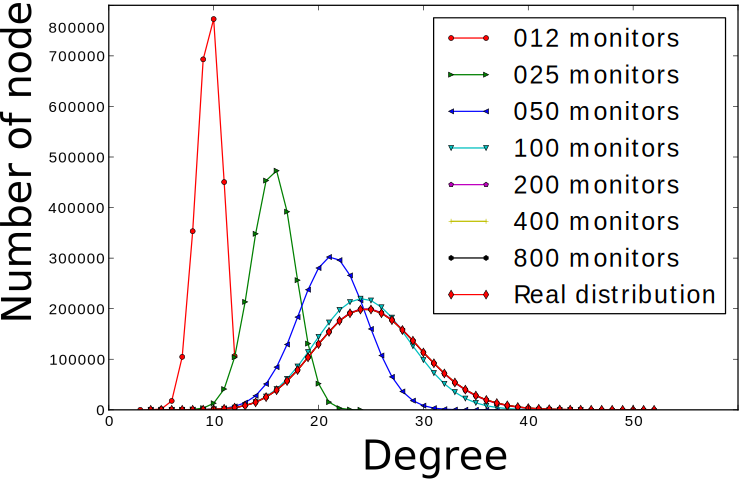
\includegraphics[width=\columnwidth]{images/udpping-simuls-poisson.eps}}
% \\
% \subfloat{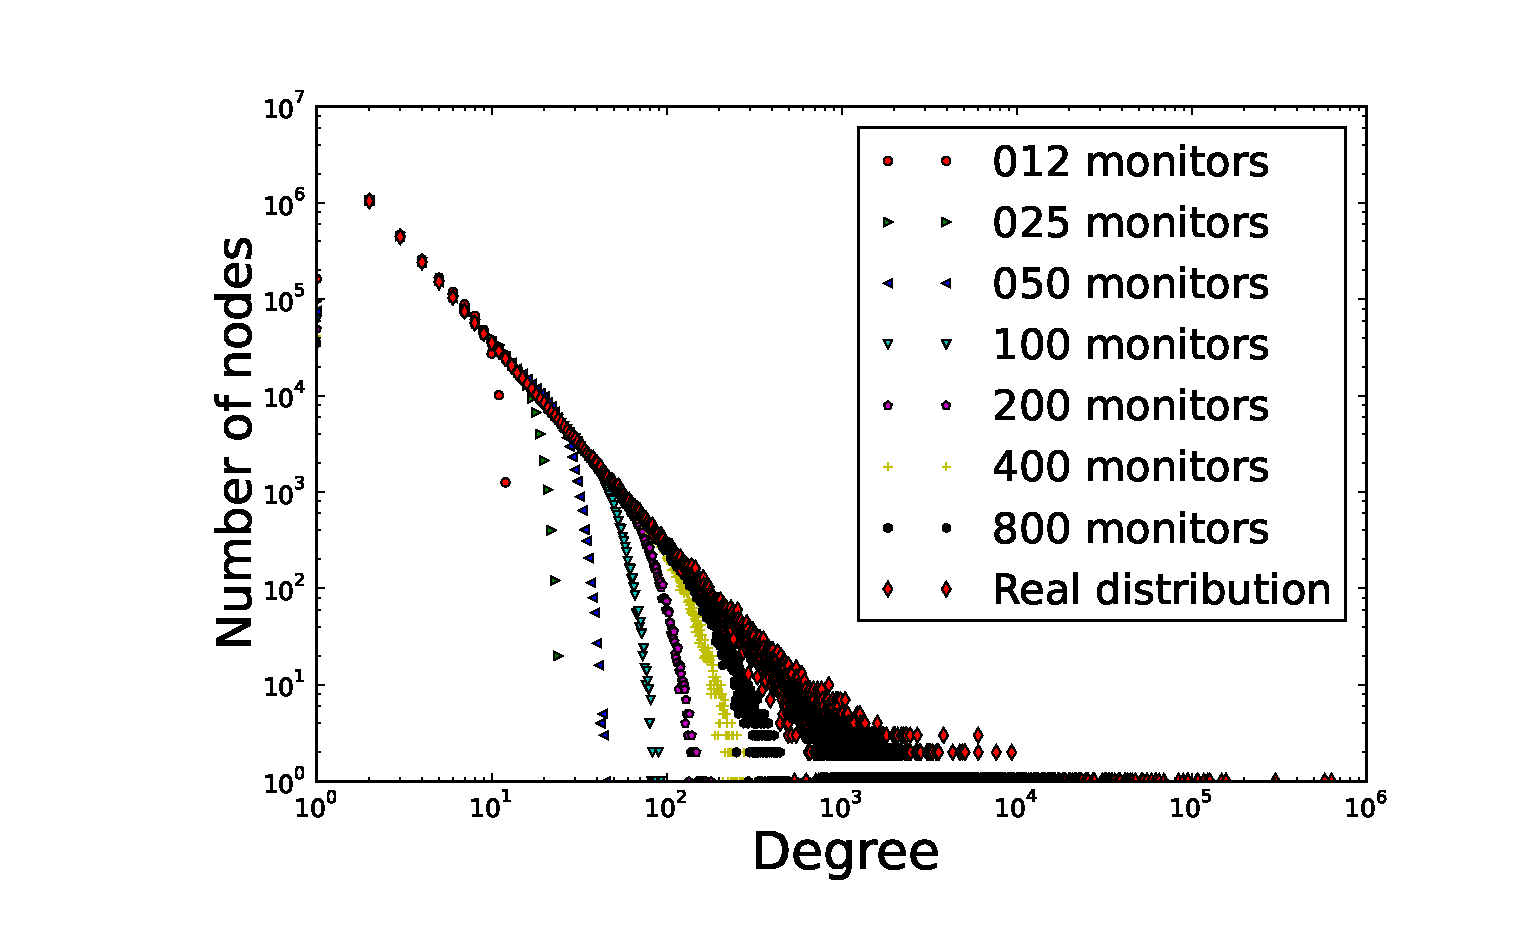
\includegraphics[width=\columnwidth]{images/udpping-simuls-powerlaw.eps}}
% \caption[Distributions de degré observées (Simulation)]{Distributions de degrés
% observées avec différents ensembles de moniteurs, et distribution réelle, dans
% le cas (en haut) d'une topologie en loi de Poisson de degré moyen $25$ et dans
% le cas (en bas) d'une topologie en loi de puissance d'exposant $2.1$ (2) ayant
% chacune $2.5*10^6$ n\oe{}uds, pour différents nombres de moniteurs ($12$, $25$, $50$, $100$, $200$,
% $400$, $800$).
% (1) En abscisse, le degré $k$, et en ordonnée, la fraction $p_k$ des n\oe{}uds
% du c\oe{}ur ayant ce degré. (b) En abscisse, le degré réel $|\overline{t}|$, et en ordonnée,
% le degré observé $|M(t)|$.}
% \label{fig:udpping-simuls}
% \end{figure}


\realfig{udpping-simuls-poisson-detail}{Observation de la distribution de
degrés, simulation avec une loi de Poisson} {Observations réalisées par la
simulation dans le cas d'une topologie en loi de Poisson de degré moyen $25$ de
$2.5*10^6$ n\oe{}uds. À gauche : la distribution réelle, en orange, et les
distributions observées pour différentes tailles de l'ensemble des moniteurs; en
abscisse, le degré $k$ et en ordonnée, la fraction $p_k$ des n\oe{}uds du
c\oe{}ur ayant ce degré. À droite : Comparaison entre les fractions de chaque
degré dans la distribution réelle et dans les distribution mesuréespour
différents nombres de moniteurs; en abscisse, le degré $k$ et en ordonnée, la
différence (en pourcentage) entre la fraction de n\oe{}uds de degré $k$ dans la
distribution réelle et dans la distribution mesurée.}
{udpping-simuls-poisson-detail}

\realfig{udpping-simuls-powerlaw-detail}{Observation de la distribution de
degrés, simulation avec une loi de puissance.} {Observations réalisées par la
simulation dans le cas d'une topologie en loi de puissance d'exposant $2.1$ de
$1.0*10^7$ n\oe{}uds. En haut à gauche : la distribution réelle, en orange, et
les distributions observées pour différentes tailles de l'ensemble des
moniteurs; en abscisse, le degré $k$ et en ordonnée, la fraction $p_k$ des
n\oe{}uds du c\oe{}ur ayant ce degré. En haut à droite : comparaison entre les
fractions de chaque degré dans la distribution réelle et dans les distributions
mesurées pour différents nombres de moniteurs; en abscisse, le degré $k$ et en
ordonnée, la différence (en pourcentage) entre la fraction de n\oe{}uds de degré
$k$ dans la distribution réelle et dans la distribution mesurée. En bas à gauche
: la distribution cumulative inverse réelle, en orange, et les distributions
cumulatives inverses observées pour différentes tailles de l'ensemble des
moniteurs. En bas à droite : zoom sur la distribution de degrés pour les faibles
degrés (inférieurs à 60) en échelle {\em lin-log}.}
{udpping-simuls-powerlaw-detail}

Ces assertions sont illustrées par la~\reffig{udpping-simuls-poisson-detail} (à
droite) et la~\reffig{udpping-simuls-powerlaw-detail} (en haut à droite). On
constate que pour $200$ moniteurs, l'estimation de {\em chacun} des n\oe{}uds,
et pas seulement de la distribution complète, est très bonne dans le cas de la
topologie homogène, ce qui démontre que notre méthode est très performante pour
ce type de graphes. Concernant la topologie en loi de Puissance, l'estimation
est excellente pour les n\oe{}uds de degré faible. Les n\oe{}uds de degré $2$,
par exemple, sont observé pour $95\%$ d'entre eux avec leur degré réel. Si l'on
étend jusqu'aux n\oe{}uds de degré $\leq 10$, alors cette proportion est de
$85\%$. Pour les n\oe{}uds de degré relativement faible, notre méthode est donc
très satisfaisante.

Le cas problématique pour notre méthode semble être l'estimation des n\oe{}uds de
fort degré des distributions hétérogènes, et en particulier les n\oe{}uds dont le
degré excède ou se rapproche du nombre total de moniteurs, $|M|$. Cependant, il
s'agit bien d'un effet de seuil, et non d'une mauvaise observation en soi. Le
nuage de points montre que les n\oe{}uds de très fort degré sont sous-évalués, mais
qu'ils ne sont pas confondus avec des n\oe{}uds de faible degré. Quel que soit le
nombre de moniteurs, la pire estimation du degré d'un n\oe{}ud degré donné (le
point le plus bas sur l'axe des ordonnées) augmente avec le degré. Pour $200$
moniteurs, par exemple, la pire estimation d'un n\oe{}ud de degré supérieur à
$1000$ l'estime comme ayant un degré de $136$.

En conclusion, dans le cas de la topologie en loi de Poisson comme dans le cas
de la topologie en loi de puissance, la nature et la forme de la distribution de
degré sont correctement observés, même avec un nombre très faible de moniteurs.
Par ailleurs, la distribution observée converge rapidement vers la distribution
réelle quand le nombre de moniteurs augmente. Le degré réel de chacun des n\oe{}uds
de faible degré (et de haut degré dans le cas d'une distribution homogène) est
correctement observé, et les n\oe{}uds de fort degré peuvent être sous-évalués,
mais jamais observés comme des n\oe{}uds de faible degré.

En dehors du cadre de cette thèse, C. Crespelle et F. Tarissan ont mené des
travaux de validation approfondis~\cite{CT01} pour explorer un grand nombre de
cas, notamment des topologies en loi de Poisson avec d'autres degrés moyens et
des topologies en loi de puissance avec d'autres exposants.
Ils ont montré que la taille totale du graphe avait très peu d'impact sur la
qualité de l'observation pour un nombre donné de moniteurs.
Ainsi, les résultats obtenus sur des graphes synthétiques de quelques millions
de n\oe{}uds restent légitimes dans le cas d'Internet dont la taille totale est
plus grande de plusieurs ordres de grandeur.

\section{Evaluation d'un ensemble de moniteurs}
\label{sec:udpping-monitors}

La qualité de l'observation du degré de chaque cible, et par conséquent de notre
estimation de la distribution de degrés, repose sur l'hypothèse que nous
disposons d'un ensemble de moniteurs adapté. Des simulations
(\refsec{udpping-simuls}) ont montré qu'un nombre relativement restreint de
moniteurs permet en principe de réaliser une estimation très précise,
mais sous l'hypothèse que ces moniteurs sont des n\oe{}uds choisis aléatoirement
parmi les n\oe{}uds de degré $1$. La simple taille de l'ensemble de moniteurs ne
suffit évidemment pas. Par exemple, avoir plusieurs moniteurs dans le même arbre
du bord peut présenter un intérêt limité, dans la mesure où leurs observations
seront souvent redondantes, puisque les chemins depuis une cible vers tous ces
moniteurs seront vraissemblablement initiés par la même interface de cette
cible. En pratique, le problème se pose plutôt dans l'autre sens :
étant donné un ensemble de moniteurs que l'on a à disposition, il faudrait
pouvoir évaluer s'il est suffisamment bien réparti pour obtenir une estimation
satisfaisante, et, éventuellement, extraire de cet ensemble de moniteurs un
sous-ensemble de moniteurs non-redondants pour éviter de réaliser des mesures
inutiles. Pour répondre à cette question, nous avons mis au point trois
approches différentes et complémentaires : la colocalisation des moniteurs
(\refsubsec{udpping-monitors-coloc}), la diversité des observations
(\refsubsec{udpping-monitors-diversity}), et la convergence des résultats
(\refsubsec{udpping-monitors-convergence}).

\subsection{Colocalisation des moniteurs}
\label{subsec:udpping-monitors-coloc}

Nous nous intéressons au cas des moniteurs situés dans le même arbre du bord,
qu'on appelle {\em moniteurs colocalisés}. Remarquons d'abord qu'un moniteur $m$
donné peut identifier quel est le n\oe{}ud du c\oe{}ur à la racine de cet arbre
:
il s'agit d'un n\oe{}ud de {\em branchement} (voir~\refsec{udpping-one-to-one}),
qui est un n\oe{}ud du c\oe{}ur dont l'une des interfaces le relie à un n\oe{}ud
du bord dont $m$ est un descendant dans cet arbre enraciné. Pour identifier ce
n\oe{}ud depuis $m$, nous avons conçu un outil très proche d'\udpping, nommé
\udpexplore, et qui procède de la manière suivante, illustrée
en~\reffig{udpping-udpexplore}.
Pour chaque distance $d$ en démarrant à 1, $m$ envoie un certain nombre $K$ de
paquets \udpping (paquet \udp arbitraire vers un port non utilisé), avec un \ttl
égal à $d$, chacun à destination d'une adresse routable aléatoire, et collecte
les paquets \icmp {\em Time Exceeded} qui sont générés à l'expiration du \ttl.
L'ensemble des adresses ayant répondu à de tels paquets est noté $d(m)$. Puisque
$m$ est une feuille d'un arbre du bord, alors {\em tous} les paquets vers une
destination aléatoire empruntent le seul chemin possible vers le reste du
graphe, c'est à dire qu'ils remontent le long de cet arbre. Soit
$\overline{d}(m)$ l'ensemble des {\em hôtes} sous-jacent à $d(m)$, calculé par
{\em anti-aliasing}. Il y a alors deux cas. Soit $\overline{d}(m)$ est réduit à
un seul hôte, auquel cas cet hôte est nécessairement l'ancêtre de rang $d$ de
$\overline{m}$ dans l'arbre du bord dont il est une feuille, soit
$\overline{d}(m)$ contient au moins deux hôtes, et alors $d$ majore la hauteur
totale de l'arbre dont il est une feuille. Le cas limite ($d_{\max}$, le dernier
$d$ tel que $|\overline{d}(m)| \leq 1$) expose l'ancêtre de rang $h$ de $m$ où
$h$ est la hauteur de l'arbre dont il est une feuille, c'est à dire que
$\overline{d}(m)$ est réduit à la racine de cet arbre, ou encore que
$\overline{d}(m)$ est le n\oe{}ud de {\em branchement} de cet arbre. Plus
précisément, on sait alors que $d(m)$ est l'unique interface de
$\overline{d}(m)$ tournées vers $m$. Dans ce cas, on note $\beta(m) = d(m)$ et
$\overline{\beta}(m) = \overline{d}(m)$.\footnote{$\beta$ pour "branchement".}
L'ensemble de {\em toutes} les interfaces observées successivement par \udpping
depuis $m$ est noté ${\mathbb B}(m) = \{ d(m), d \leq d_{\max} \}$.

Notons qu'il se peut qu'\udpexplore n'obtienne aucun résultat pour une distance
$d$ donnée, pour les mêmes raisons que \udpping peut ne pas obtenir de réponse,
par exemple à cause du filtrage \icmp ou d'un {\em firewall} sur l'un des hôtes
traversés. Ceci n'est pas tellement problématique, sauf dans le cas où aucune
réponse n'est obtenue pour le dernier $d$ tel que $|\overline{d}(m)| \leq 1$.
Dans ce cas, on ne connaît pas $\beta(m)$.

\realfig{udpping-udpexplore.png}{\udpexplore --- n\oe{}ud de branchement d'un
moniteur} {Le moniteur $m$ est une feuille d'un arbre enraciné dont la racine
est un n\oe{}ud du c\oe{}ur. Les sondes \udpexplore (parcourant les liens et les
n\oe{}uds en noir) permettent d'identifier tous les ancêtres de $\overline{m}$ dans
cet arbre, et en particulier de trouver la racine $\overline{\beta}(m)$ en
les énumérant.}{udpping-udpexplore}

Soit alors $m$ et $m'$ deux moniteurs quelconques. Alors $m$ et $m'$ sont dans
le même arbre du bord si et seulement si $\overline{\beta}(m) =
\overline{\beta}(m')$. Donc pour décider si $m$ et $m'$ sont dans le même arbre,
il suffit d'exécuter \udpexplore depuis $m$ et depuis $m'$ et d'effectuer un
test d'{\em anti-aliasing} entre leurs résultats.

\realfig{udpping-coloc.png}{Moniteurs colocalisés}{$m_2$ et $m_3$ sont
dans le même arbre du bord, et tous les chemins depuis le c\oe{}ur vers n'importe lequel d'entre deux
passe par leur n\oe{}ud de {\em branchement} $\overline{\beta(m_2)} =
\overline{\beta(m_3)}$.
Par exemple, le n\oe{}ud $\overline{t}$ utilise la même interface $t'$ pour leur
répondre, alors qu'il utilise son interface $t$ pour répondre à un autre
moniteur $m_3$ situé dans un autre arbre du bord, de racine
$\overline{\beta(m_1)}$.}{udpping-coloc}

Cette notion de moniteur colocalisé nous permet d'exprimer la notion intuitive
correspondant à deux routeurs {\em proches} et donc susceptibles de réaliser des
observations identiques, c'est à dire telles que les cibles observées utilisent
la même interface pour leur répondre (\reffig{udpping-coloc}). Notre
méthode pour les détecter est inclusive, c'est à dire que deux moniteurs non
colocalisés ne seront jamais identifiés comme tels. En revanche, deux moniteurs
colocalisés peuvent éventuellement ne pas être détectés comme tels, par exemple
si les hôtes sur les chemins vers le c\oe{}ur d'un moniteur ne répondent pas aux
sondes \udpping, et ne permettent pas de conclure.

\udpexplore est également utilisé pour effectuer la transformation $\varphi_2$
décrite en ~\refsec{udpping-many-to-many}. Pour chaque moniteur
$m$, $m$ est susceptible d'observer une interface $t$ de $\overline{t}$ qui
n'est pas dans le c\oe{}ur si et seulement si, $t \in {\mathbb B}(m)$. Cette
assertion est valable même si \udpexplore n'obtient pas de réponses. En effet,
dans un tel cas, $\overline{t}$ filtre le traffic \icmp ou \udp sur
l'interface $t$, ce qui empêche \udpexplore de fournir un résultat, mais
également \udpping de réaliser une observation invalide d'une
interface qui ne serait pas dans le c\oe{}ur. Plus généralement, pour un ensemble
de moniteurs $M$, une interface $t$ d'une cible qui ne serait pas une interface
du c\oe{}ur ne peut être observée que si $t \in {\mathbb B}(M)$ avec ${\mathbb
B}(M) = \cup_{m \in M} {\mathbb B}(m)$\footnote{Ce qui justifie notre notation
${\mathbb B}$ pour {\em border blacklist}, c'est à dire une {\em liste noire}
d'interfaces potentiellement observables alors qu'elles ne sont pas dans le
c\oe{}ur mais dans le bord.}.

Grâce aux résultats d'\udpexplore, nous pouvons définir une notion de qualité
\emph{intrinsèque} d'un ensemble de moniteurs, correspondant à l'ensemble des
emplacements topologiquement distincts représentés dans l'ensemble, et pouvant
potentiellement mener à des observations d'interfaces différentes au moins pour
certaines cibles. Cette qualité intrinsèque est définie par rapport à l'ensemble
total de ces emplacements, et s'exprime en termes d'ensembles-quotients de la
relation d'équivalence induite par $\beta$. Un \emph{emplacement dans le réseau}
est une classe d'équivalence sur l'ensemble $L_3$ pour la relation d'égalité sur
le critère $\beta$, c'est à dire pour la relation $v \equiv u \Leftrightarrow
\beta(v) = \beta(u)$. On considère l'ensemble-quotient $L_3/\equiv$. La
\emph{qualité intrinsèque} d'un ensemble de moniteurs $M$ est alors définie par
$M/\equiv$ (plongé dans $L_3/\equiv$).

Toutes les classes n'ont pas la même valeur pour ce qui est de l'apport à
l'observation, mais en première approximation, on peut s'intéresser à la
\emph{taille} du quotient $|M/\equiv|$ pour évaluer la qualité intrisèque de
$M$.

\subsection{Diversité des observations}
\label{subsec:udpping-monitors-diversity}

La notion de moniteurs colocalisés nous permet d'exprimer une qualité
intrinsèque d'un ensemble de moniteurs, comme une sorte de "degré de liberté"
\apriori de notre ensemble correspondant au nombre d'emplacements
topologiquement distincts dans notre ensemble de moniteurs (les classes
d'équivalences induites par $\beta$). Un point de vue plus pragmatique et
complémentaire consiste à s'intéresser \aposteriori à la \emph{diversité des
observations} obtenues pour une mesure d'un ensemble de cibles $T$ par un
ensemble de moniteurs $M$. Pour ce faire, nous nous fixons une \emph{fonction
de qualité} $Q : (T, M) \mapsto Q(T, M) \in {\mathbb R}$, qui définit une
évaluation de la diversité des observations, et doit respecter quelques
critères qui correspondent à l'intuition :

\begin{itemize}
  \item Un ensemble de cibles ou de moniteurs vide a une qualité nulle :
  \begin{equation}
  Q(\emptyset, M) = Q(T, \emptyset) = 0
  \end{equation}
  \item La qualité est croissante par ajout de moniteurs :
  \begin{equation}
  \label{eq:udpping-monitors-diversity-add-monitors}   
  Q(T, M \cup \{ m \}) \geq Q(T, M)
  \end{equation}
  \item La qualité est au minimum conservée par fusion d'ensemble de cibles pour
  un ensemble de moniteurs fixé :
  \begin{equation}
  \label{eq:udpping-monitors-diversity-merge-targets}
  Q(T \cup T', M) \geq {\min}(Q(T, M), Q(T', M))
  \end{equation}
%   \item La qualité est croissante par ajout de cibles :
%   \begin{equation}
%   Q(T \cup \{ t \}, M) \geq Q(T, M)
%   \end{equation}
  \item La qualité réduite à une cible unique est croissante par ajout
  d'interfaces observées :
  \begin{equation}
  |\overline{M(t)}| \geq |\overline{M'(t)}| \Rightarrow Q(\{ t \}, M) \geq
  Q(\{ t \}, M')
  \end{equation}
\end{itemize}

Par exemple, on peut se contenter de compter le nombre
d'interfaces distinctes observées au total, c'est-à-dire $Q_0(T, M) = \sum_{t
\in T} | \overline{M(t)} |$. Alors, dans ce cas, pour deux ensembles de moniteurs
$M$ et $M'$, et si $Q_0(T, M') > Q_0(T, M)$, on peut considérer que $M'$
est \emph{meilleur} que $M$ en ce sens qu'il observe davantage d'interfaces
des cibles.

On peut utiliser une fonction de qualité plus subtile, par exemple pour prendre
en compte le fait que chaque interface d'un n\oe{}ud de faible degré est
vraissemblablement plus facile à observer que les interfaces d'un n\oe{}ud de fort
degré. En effet, supposons pour simplifier que pour un n\oe{}ud de degré $d$,
chacune de ses interfaces est observée avec une probabilité $\frac{1}{d}$. Alors
en moyenne pour $N$ moniteurs indépendants\footnote{Ce qui est bien sûr
également une simplification puisque c'est cette indépendance que nous
cherchons à approcher.} tirés aléatoirement, une interface d'un n\oe{}ud de
degré $d$ sera observé par $\frac{N}{d}$ moniteurs. Pour contrebalancer ce facteur, on
peut utiliser la fonction de qualité $Q_1$ définie par $Q_1(T, M) = \sum_{t \in
T} |\overline{M(t)}|d(t)$ où $d(t)$ est le degré de $t$, qui est ici approximé par
$|\overline{M(t)}|$, ce qui donne $Q_1(T, M) \simeq \sum_{t \in T}
|\overline{M(t)}|^2$.


Une fonction de qualité est également majorée, pour un ensemble de cibles
$T$ donné, par le cas idéal où \emph{tous les n\oe{}uds du réseau sont des
moniteurs}, auquel cas \emph{toutes les interfaces de toutes les cibles sont
observées}. On peut éventuellement utiliser cette notion pour normaliser
théoriquement la qualité, même si ce facteur de normalisation n'est pas vraiment
calculable en pratique :
$$Q^* : (T, M) \mapsto \frac{Q(T, M)}{Q(T, L_3)} \in [0, 1]$$

Pour une fonction de qualité $Q$ telle que décrite ci-dessus, on peut
calculer l'impact de l'\emph{ajout} d'un nouveau moniteur $m$ à un ensemble
de moniteurs $M$, en calculant $\Delta Q(T, M, \{ m \}) = Q(M \cup \{ m \}) -
Q(M)$ (qui est une valeur positive
d'après l'hypothèse~\ref{eq:udpping-monitors-diversity-add-monitors}).
Idéalement, on souhaite maximiser $\Delta$ à chaque ajout de moniteur, pour
augmenter la qualité de $M$ tout en minimisant sa taille de manière gloutonne,
pour limiter la charge imposée au réseau par la mesure.

D'après les simulations effectuées en
~\refsec{udpping-simuls}, on s'attend à ce que $Q$ se rapproche
rapidement de sa valeur maximale, c'est à dire à ce que $Q^*$ se rapproche
rapidement de 1 à mesure que $M$ grandit, sauf bien sûr si l'on rajoute des
moniteurs qui n'augmentent pas la fonction de qualité --- c'est à dire s'ils
sont colocalisés, et c'est pour cette raison que cette approche est
\emph{complémentaire} à l'approche de la colocalisation. En particulier, on peut
combiner les deux approches en réduisant un ensemble de moniteurs $M$ à son
quotient $M/\equiv$ et en sélectionnant un représentant de chacune des classes
pour étendre une fonction de qualité à un ensemble d'\emph{emplacements du
réseau} au lieu d'un ensemble de moniteurs. Cette approche combinée possède
plusieurs avantages : tout d'abord, elle permet de répondre à la question
soulevée auparavant des valeurs relatives des emplacements du réseau; et elle permet
d'utiliser la colocalisation pour avoir une approche plus fine que l'approche
gloutonne pour optimiser la qualité d'un ensemble de moniteurs. Enfin, elle
permet de vérifier la pertinence de chacune des approches, en s'assurant
qu'augmenter le nombre d'emplacements augmente bien la qualité d'un ensemble de
moniteurs, et qu'ajouter des moniteurs déjà colocalisés ne l'augmente pas (ou
peu).

Cependant, il n'est pas courant qu'on puisse arbitrairement étendre l'ensemble
des moniteurs, \afortiori avoir le loisir de choisir un moniteur supplémentaire
optimal (en maximisant sa contribution à la qualité). En pratique, on utilisera
cette notion non pas pour améliorer la qualité d'un ensemble donné, mais pour
décider si un ensemble de moniteurs donné est de \emph{suffisamment bonne
qualité}. Pour ce faire, nous exploitons le fait que lorsque l'ensemble des
moniteurs atteint une qualité suffisante, sa qualité $Q$ est proche de la valeur
maximale, c'est à dire que sa qualité normalisée $Q^*$ est proche de 1. Après
une mesure réelle, on injecte les résultats de la mesure, filtrés par des
ensembles croissants de moniteurs ajoutés dans un ordre aléatoire, $\emptyset =
M_0 \subset M_1 \subset \ldots M_{n-1} \subset M_n \subset M_{n+1} \ldots
\subset M_{|M| - 1} \subset M_{|M|} = M$, depuis l'ensemble vide $\emptyset$
jusqu'à l'ensemble de tous les moniteurs $M$, et on calcule la qualité de chaque
$Q(M_n)$.

Si $M$ est suffisamment grand et suffisamment bien réparti, alors on s'attend à
ce que la courbe $n \mapsto Q(M_n)$ atteigne un régime stationnaire, à partir
duquel $Q(M_n)$ est très proche de $Q(M)$. Notons que malheureusement la
réciproque n'est pas vraie. Si $n \mapsto Q(M)$ atteint un régime stationnaire,
cela ne signifie pas nécessairement que $M$ est assez grand. En effet, si par
exemple $M$ est composé d'un très petit nombre de moniteurs à des emplacements
distincts et d'énormément de moniteurs colocalisés, alors on s'attend à ce que
$Q(M_n)$ atteigne rapidement un régime stationnaire, sans pour autant être assez
grand et bien réparti. Cette approche permet donc de valider (ou d'invalider)
qu'un ensemble de moniteurs est optimal \emph{localement}, c'est à dire qu'en
rajoutant des moniteurs qui sont informellement \emph{de même nature}, par
exemple "appartenant à l'ensemble des hôtes de \planetlab", on n'améliore plus la
qualité de l'ensemble des moniteurs.

\subsection{Convergence des résultats}
\label{subsec:udpping-monitors-convergence}

Une dernière approche, semblable à celle des fonctions de qualité, consiste à
s'intéresser non plus aux détails de notre mesure, mais à son résultat final,
c'est à dire les fractions de n\oe{}uds ayant un degré observé donné $p_k$. Cette
interprétation peut être vue comme un cas particulier d'une fonction de qualité
normalisée particulière, définie de la manière suivante pour $M' \subset M$ :
$$Q_{p_k}(T, M') = |\{ t \in T, |\overline{M'(t)}| = k \}|$$

Soit, en normalisant :

$$Q^*_{p_k}(T, M') = \frac{p_k(M')}{p_k}$$

où $p_k(M')$ est la fraction de moniteurs observés avec un degré $k$ en
utilisant les moniteurs de $M'$.

Là encore, on s'attend à ce que cette fraction converge rapidement si l'ensemble
$M$ est assez grand et assez bien réparti. L'avantage de cette approche
particulière est surtout conceptuel, dans la mesure où le critère de validation
est directement lié au résultat final auquel on s'intéresse et s'abstrait des
détails de l'implémentation.

Tout comme pour la fonction de qualité, ce calcul peut être raffiné en
s'intéressant non pas à tous les moniteurs successifs, mais en se restreignant à
un représentant par classe d'équivalence pour la relation de colocalisation
$\equiv$.

\section{Mesure réelle}
\label{sec:udpping-measurement}

Nous avons réalisé une mesure réelle pour mettre à l'épreuve notre méthode de
mesure. Les objectifs étaient multiples. Le premier est bien sûr d'attester de
la faisabilité pratique de notre méthode. L'un des enjeux majeurs à ce niveau
concerne le filtrage des résultats, qui présente \apriori le risque de supprimer
tellement de données que la quantité fiable restante serait trop faible pour
effectuer une estimation du résultat. Cette mesure devait également nous
permettre d'éprouver nos méthodes théoriques de validation des résultats, qui
reposent sur des données concrètes et s'effectuent \aposteriori. Enfin, elle
devait nous donner un aperçu du résultat, fût-il sur un ensemble de moniteurs
très particulier (en l'occurence \planetlab).

Nous allons présenter dans cette section les conditions du déroulement de notre
mesure réelle (\refsubsec{udpping-measurement-setup}), et les résultats
que nous avons obtenus (\refsubsec{udpping-measurement-results}). Les
données issues de cette expérimentation seront également mobilisées
en~\refsec{udpping-validation} pour mettre à l'épreuve nos méthodes de
validation.

\subsection{Déroulement}
\label{subsec:udpping-measurement-setup}

Notre mesure s'est déroulée en plusieurs étapes distinctes : la constitution
d'une liste initiale de cibles, l'exécution d'\udpping depuis chaque moniteur
vers chaque cible, l'exécution d'\udpexplore depuis chaque moniteur, et
l'analyse et le filtrage des données collectées. Afin de limiter l'impact de la
dynamique du réseau, nous avons enchaîné les 3 premières étapes.

La constitution de la liste correspond en partie à la méthode décrite en
~\refsubsec{udpping-many-to-many-addresses}. Cependant, les filtrages
$\varphi_2$ et $\varphi_3$ ne peuvent être complètement réalisés au fur et à
mesure de la constitution de la liste et nécessitent d'avoir déjà réalisé la
mesure \udpping et la mesure \udpexplore. Nous pouvons donc choisir de
constituer la liste de telle sorte qu'après $\varphi_1$, on ait un nombre
arbitraire de cibles restantes, mais il faut la constituer assez grande pour
qu'après les filtrages ultérieurs, $T = \varphi(T_0)$ soit assez suffisamment
grand.

Nous avons donc tiré des adresses \ip (entiers 32 bits) de manière
uniformément aléatoire successivement jusqu'à obtenir $N = 3 \times 10^6$
adresses qui étaient des adresses \emph{valides et routables}, et surtout, qui
\emph{répondent aux sondes \udpping}, en envoyant une sonde isolée depuis un
unique moniteur. L'ensemble obtenu correspond directement à $T_1 =
\varphi_0(T_0)$, et nous avons arrêté le procédé lorsque nous avions atteint
$|T_1| = N$. Cette opération, réalisée depuis un unique moniteur de notre
ensemble, a duré environ 10 heures. Notons que par simplicité, nous avons
réalisé ce tirage depuis un moniteur unique, mais que nous pouvons énormément
accélérer ce processus en distribuant le tirage (et surtout l'exécution
d'\udpping associée) sur plusieurs moniteurs.

Notre ensemble de moniteurs initial $M_0$ était composé d'environ $K = 700$
machines de la plateforme \planetlab~\cite{planetlab}. Certains de ces moniteurs
n'étaient pas exploitables, à cause de problèmes de connectivité par exemple, ou
étaient colocalisés entre eux, mais ces considérations ont été gérées
\aposteriori afin de réaliser une collecte aussi large que possible.

Nous avons envoyé notre outil \udpping pré-compilé sur chacun de ces moniteurs,
ainsi qu'une liste des cibles $T_1$, mélangée dans un ordre aléatoirement choisi
pour chacun des moniteurs. Ce mélange est destiné à limiter dans une certaine
mesure l'envoi simultané de très nombreuses sondes vers une unique cible, même
si cette méthode est assez rudimentaire. Une fois la mise en place terminée, la
mesure \udpping à proprement parler a pu avoir lieu, et a duré environ 4
heures.
Durant ces 4h, chaque cible a en principe reçu au maximum $K = 700$ sondes
\udpping, et chaque moniteur a émis au maximum $N = 3 \times 10^6$ sondes
\udpping. Afin de nous permettre d'étudier la stabilité de la mesure, la mesure
\udpping a été répétée 3 fois à la suite. L'exécution d'\udpexplore depuis
chaque moniteur s'est déroulée en quelques minutes. Au total, avec la création
de la liste de cibles (l'opération la plus longue), les 3 prélèvements \udpping
et le prélèvement \udpexplore, l'opération s'est déroulée sur moins de 24h, et
n'a fait supporter aux cibles et à leur voisinage qu'une charge très modérée de
quelques centaines de paquets \udp. À ce stade, nous avons rappatrié toutes les
données mesurées (\udpping et \udpexplore) sur une machine locale pour procéder
à l'analyse \aposteriori.

\begin{table}[!ht]
\centering
\begin{tabular}{|c|c|c|c|}
\hline
										& Itération 1	& Itération 2	& Itération 3 \\
\hline
$|M_0|$									& 619			& 625			& 622 \\
\hline
$|M|$									& 421			& 442			& 442 \\
\hline
$|{\mathbb B}(M)|$						& 1040			& 1107			& 1097 \\
\hline
$|T_1|$									& 2849740		& 2734548 		& 2699642 \\
\hline
$|T_1| - |\varphi_1'(T_1)|$				& 10150			& 9842			& 11048 \\
\hline
$|T_1| - |\varphi_1''(T_1)|$			& 590605		& 527346		& 544252 \\
\hline 
$|T_1| - |\varphi_1^*(T_1)|$			& 600755		& 537188		& 555300 \\
\hline
$|T_1| - |\varphi_2(T_1)|$				& 2842281		& 2727422		& 2692135 \\
\hline
$|T_1| - |\varphi_3(T_1)|$				& 2634226		& 2519320		& 2488483 \\
\hline
$|T|$									& 5593			& 5623			& 5619 \\
\hline						
\end{tabular}
\caption[Filtrage des données après la mesure]{Filtrage des données après la
mesure.}
\label{table:udpping-measurement-filtering}
\end{table}

L'analyse a démarré par l'application pragmatique des filtres décrits
précédemment. Leur effet quantitatif est récapitulé dans
le~\reftable{udpping-measurement-filtering}. Pour \udpping, le résultat d'un
prélèvement prend la forme, pour chaque moniteur $m$, d'une liste de couples
$(t, m(t))$, où $m(t)$ est l'adresse de l'interface \emph{Source} du paquet
\icmp \emph{Destination Unreachable (Code 3/Port Unreachable)}
(voir~\refsec{udpping-one-to-one}), pour chaque paquet de ce type reçu par un
moniteur. Quelques aberrations ont été constatées, comme par exemple des
réponses multiples de la part de certaines cibles pour une sonde unique.
D'autres cibles n'ont répondu qu'à un nombre très limité de moniteurs,
probablement à cause d'une disponibilité limitée pendant la durée de la mesure,
ou d'une limitation forte du trafic \icmp ({\em rate limiting}). De même,
certains moniteurs n'ont obtenu que très peu de réponses, soit à cause d'une
connectivité locale très faible, une disponibilité limitée, ou une surcharge au
niveau de l'hôte \planetlab (puisque les hôtes \planetlab sont partagés entre de
nombreux utilisateurs). Pour éviter toute anomalie liée à ces problèmes
techniques, nous avons d'abord supprimé de notre jeu de données les cibles
donnant au moins une réponse multiple, filtrage que nous notons $\varphi_1'$.
Puis, nous avons compté pour chaque moniteur, le nombre de cibles ayant fourni
une réponse, et pour chaque cible, le nombre de moniteurs les ayant observé, et
nous nous sommes intéressés à la distribution de ces valeurs
(\reffig{udpping-measurement-purification}).
Comme attendu, {\em la plupart} des moniteurs observent {\em la plupart} des
cibles, et {\em la plupart} des cibles sont observées par {\em la plupart} des
moniteurs. Pour purifier notre jeu de données, nous avons supprimé tous les
moniteurs observant moins de 80\% des cibles (les moniteurs restant définissent
l'ensemble $M = M_1$), et toutes les cibles observées par moins de 80\% des
moniteurs (filtrage $\varphi_1''$). Le filtrage correspondant à la suppression
de cibles pour leur manque de réponses est une extension de
$\varphi_1$, que l'on note $\varphi_1^* = \varphi_1'' \circ \varphi_1' \circ
\varphi_1$ de telle sorte que $T_1^* = \varphi_1^*(T_0) = \varphi_1'' \circ
\varphi_1'(T_1)$ puisque $T_1 = \varphi_1(T_0)$.

Pour procéder à la suite du filtrage et exécuter $\varphi_2$, nous avons d'abord
dû calculer ${\mathbb B}(M)$, qui est une simple reformulation des résultats
fournis par \udpping. Une fois ${\mathbb B}(M)$ calculé, nous avons supprimé
chacune des interfaces apparaissant dans cette liste de nos données, puis compté
le nombre d'interfaces observées {\em restantes} pour chaque cible.
L'application de $\varphi_2$ correspond à la supression des cibles tel que ce
nombre est égal à 0 ou 1. $\varphi_3$ est une transformation plus directe,
puisqu'elle consiste simplement à éliminer toutes les cibles $t$ telles que $t
\notin M(t)$.

En pratique, nous avons profité de la commutativité\footnote{Cette commutativé
est simplement due à la commutativité de l'intersection d'ensembles.} des
transformations $(\varphi_k)$ et appliqué ces transformations séparément à $T_1$
et réalisé l'intersection à la fin de la démarche, de telle sorte que $T =
\varphi_1'(T_1) \cap \varphi_1''(T_1) \cap \varphi_2(T_1) \cap \varphi_3(T_1) =
\varphi_3 \circ \varphi_2 \circ \varphi_1^*(T_0)$.

À l'issue de tous ces filtrages, pour chacune de nos itérations, nous observons
environ 5600 cibles. Ces cibles sont garanties, d'après notre méthode, d'être un
ensemble d'adresses d'interfaces choisies uniformément aléatoirement dans le
c\oe{}ur de routeurs du c\oe{}ur, dont nous disposons de la liste de toutes les
interfaces dans le c\oe{}ur observable par l'ensemble des moniteurs de
\planetlab.

\begin{figure}[!ht]\centering
\subfloat{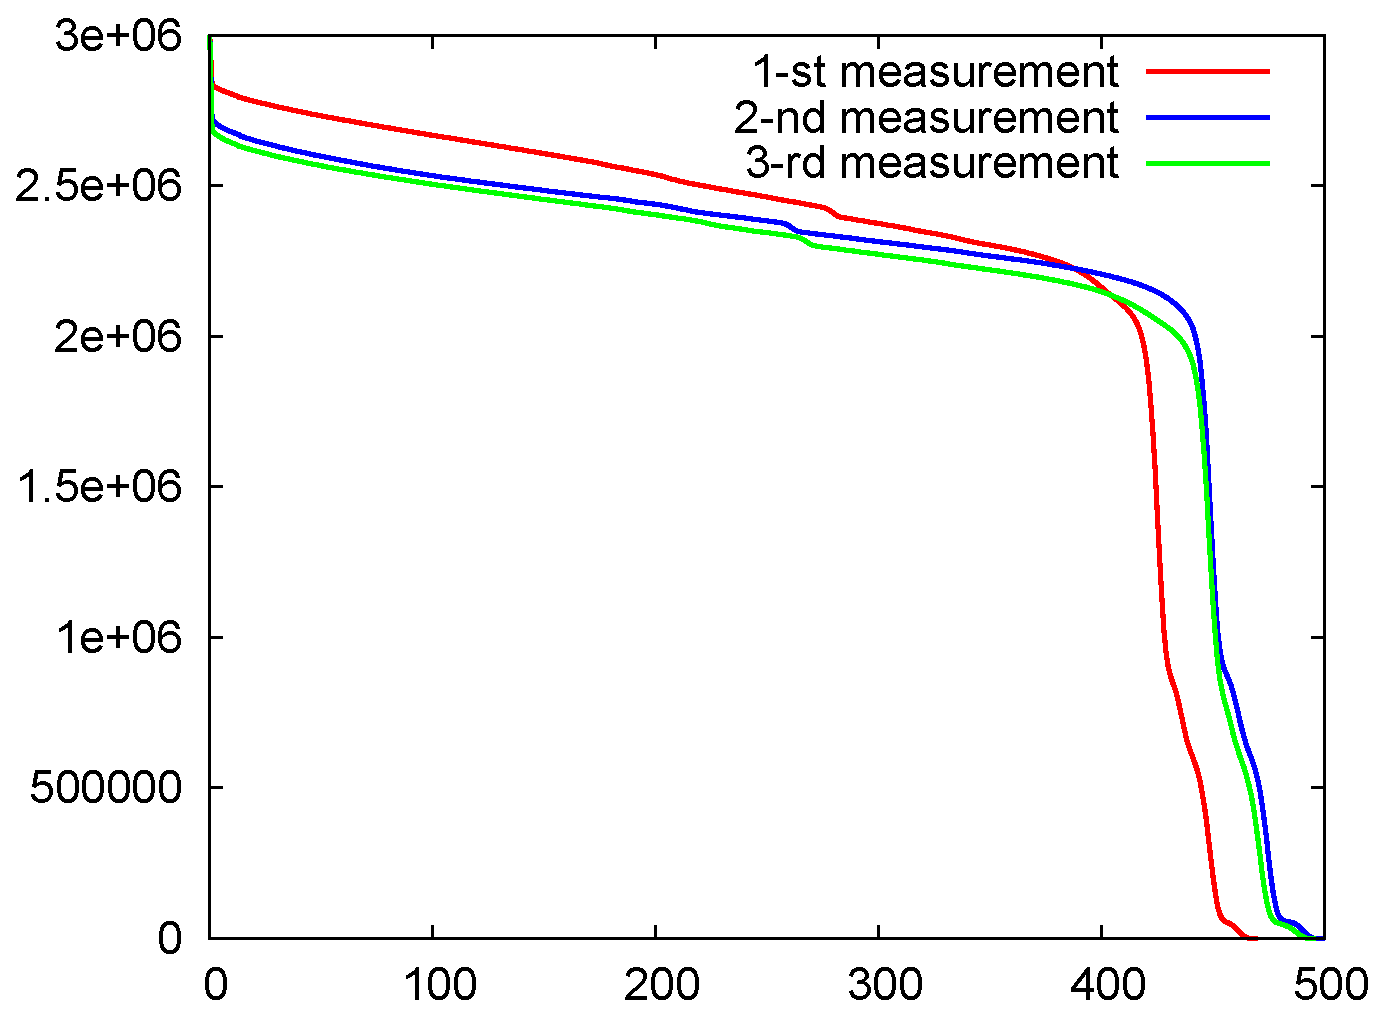
\includegraphics[width=0.9\columnwidth]{images/udpping-filter-targets.eps}}
\\
\subfloat{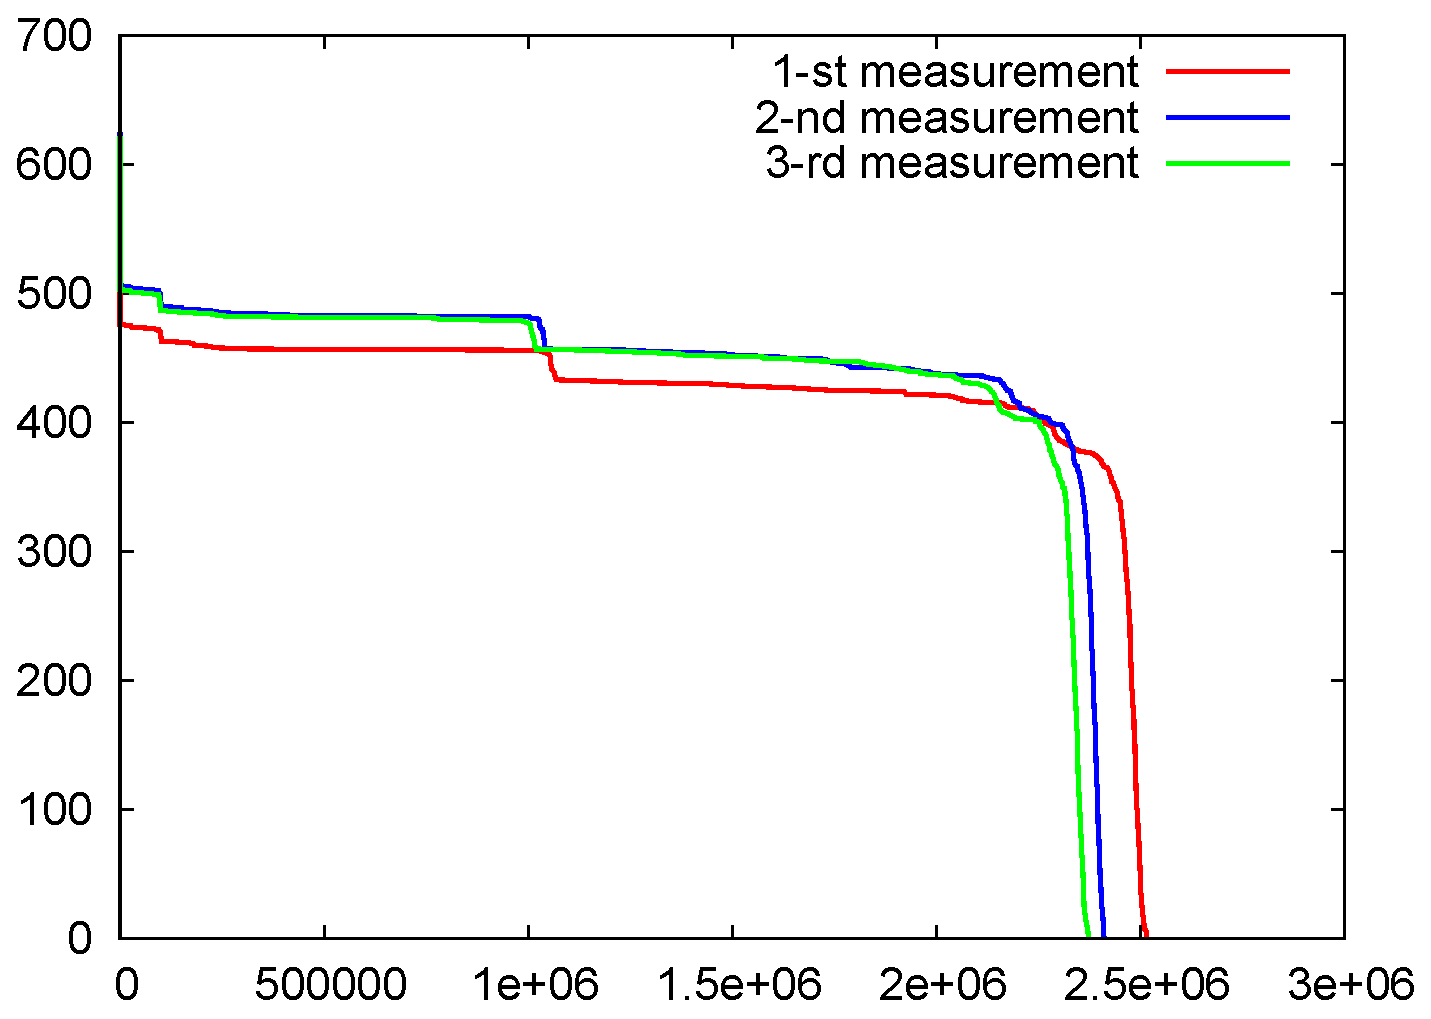
\includegraphics[width=0.9\columnwidth]{images/udpping-filter-monitors.eps}}
\caption[Nombre d'observations par cible et par moniteur]{En haut (resp. en
bas) : pour chaque $x$ sur l'axe des abscisses, nous traçons le nombre de cibles
(resp. de moniteurs) ayant envoyé (resp. reçu) au moins $x$ réponses \icmp lors
de notre mesure, pour chacune des 3 itérations.}
\label{fig:udpping-measurement-purification}
\end{figure}

\subsection{Résultats}
\label{subsec:udpping-measurement-results}

Le résultat de notre mesure prend la forme d'une liste de triplets $(m, t,
m(t))$ où $m$ décrit $M$ et $t$ décrit $T$ de telle sorte que $m(t)$ est
l'interface observée par $m$ pour la cible $t$ losqu'une réponse a été obtenue
pour le couple $(m, t)$ (ce qui est garanti d'arriver dans au moins 80\% des
cas pour chaque moniteur et pour chaque cible, à cause du filtrage que nous
avons effectué précédemment). Pour chaque cible $t$, on calcule l'ensemble
$M(t) = \{ m(t), m \in M \}$, et en particulier $|M(t)|$, qui correspond au
degré dans le c\oe{}ur observé de la cible $\overline{t}$. Pour chaque entier $k$,
on calcule ensuite la fraction $p'_k$ de cibles ayant un degré observé égal à
$k$. Cette fraction est biaisée linéairement par le degré, comme décrit
en~\refsec{udpping-many-to-many}, et on corrige ce biais en appliquant la
transformation $p'_k \mapsto \frac{p'_k}{k}$ puis en normalisant cette fraction
entre 0 et 1. Le~\reftable{udpping-measurement-results-fraction} indique les
valeurs des $(p_k)$ pour nos 3 mesures, qui sont combinées sous la forme d'une distribution
cumulative inverse en~\reffig{udpping-measurement-results-distrib}.


\begin{table}[!ht]
\centering
\resizebox{\columnwidth}{!}{
\begin{tabular}{|c|c|c|c|}
\hline
Degré $k$	& Fraction $p_k$ (Itération 1)	& Fraction $p_k$ (Itération 2)	&
Fraction $p_k$ (Itération 3) \\  
\hline
2  & 0.74770 & 0.74371 & 0.75214 \\
3  & 0.19434 & 0.19838 & 0.19258 \\
4  & 0.02727 & 0.02727 & 0.02585 \\
5  & 0.01551 & 0.01588 & 0.01486 \\
6  & 0.00708 & 0.00640 & 0.00644 \\
7  & 0.00206 & 0.00224 & 0.00230 \\
8  & 0.00175 & 0.00196 & 0.00147 \\
9  & 0.00127 & 0.00131 & 0.00145 \\
10 & 0.00057 & 0.00044 & 0.00052 \\
11 & 0.00056 & 0.00052 & 0.00047 \\
12 & 0.00040 & 0.00044 & 0.00047 \\
13 & 0.00020 & 0.00023 & 0.00017 \\
14 & 0.00025 & 0.00031 & 0.00031 \\
15 & 0.00032 & 0.00009 & 0.00017 \\
16 & 0.00014 & 0.00025 & 0.00024 \\
17 & 0.00023 & 0.00018 & 0.00015 \\
18 & 0.00007 & 0.00007 & 0.00007 \\
19 & 0.00007 & 0.00009 & 0.00009 \\
20 & 0.00002 & 0.00000 & 0.00002 \\
21 & 0.00008 & 0.00015 & 0.00008 \\
22 & 0.00006 & 0.00000 & 0.00004 \\
23 & 0.00000 & 0.00000 & 0.00002 \\
24 & 0.00002 & 0.00000 & 0.00002 \\
25 & 0.00000 & 0.00005 & 0.00002 \\
26 & 0.00000 & 0.00002 & 0.00002 \\
27 & 0.00002 & 0.00000 & 0.00002 \\
28 & 0.00000 & 0.00002 & 0.00000 \\
29 & 0.00002 & 0.00000 & 0.00001 \\
\hline						
\end{tabular}
}
\caption[Fractions des routeurs du c\oe{}ur de degré $k$]{Fractions des routeurs
du c\oe{}ur de degré $k$, après correction du biais de sélection.}
\label{table:udpping-measurement-results-fraction}
\end{table}

\realfig{udpping-measurement-results-distrib}{Distribution cumulative inverse du
degré des routeurs du c\oe{}ur}{Pour chaque valeur $x$ en abscisse, on trace la
fraction des routeurs du c\oe{}ur ayant un degré supérieur ou égal à $x$, en
échelle log-log.}{udpping-measurement-results-distrib}

Notre première observation porte sur la stabilité des résultats, c'est à dire
que les 3 itérations de notre mesure donnent des résultats très similaires, ce
qui tend à confirmer que l'échelle de temps (quelques heures) sur laquelle nous
avons effectué notre mesure n'est pas excessive.

Les distributions observées montrent clairement que les n\oe{}uds de faible degré
ont une énorme prévalence, puisqu'environ 75\% des n\oe{}uds sont de degré 2, et
environ 95\% ont un degré égal à 2 ou 3. Ce n'est pas choquant, puisque
nous nous intéressons ici uniquement aux interfaces dans le c\oe{}ur, c'est à dire
les interfaces utilisées par les routeurs pour router vers des destinations qui
ne sont pas dans un sous-réseau du bord qui leur serait rattaché, mais bien pour
effectuer un véritable {\em routage}.

Pourtant, nous observons quelques routeurs de fort degré, et le degré maximal
que nous observons est 29, pour une cible. Il est possible que nous n'observions
pas certaines de ses interfaces, mais il est peu probable que son degré réel
soit beaucoup plus élevé, puisque le nombre de moniteurs que nous utilisons
($|M| > 400$) dépasse amplement ce nombre. Cette remarque sera approfondie
en~\refsec{udpping-validation}. Il est bien sûr également possible, et probable,
que des routeurs de degré supérieur à 29 existent, mais il n'y en a aucun dans
l'ensemble que nous avons mesuré, et on s'attend donc à ce qu'ils soient
extrêmement rares sur Internet --- une hypothèse renforcée par le biais de
sélection en faveur des n\oe{}uds de fort degré.

\section{Protocole complet}
\label{sec:udpping-protocol}

Cette section fait office de synthèse de notre protocole complet pour évaluer
la distribution de degrés dans le c\oe{}ur des routeurs du c\oe{}ur, étant donné
un ensemble de moniteurs, et elle intègre à la fois la méthode théorique telle que
nous l'avons déjà décrite, et les ajustements opérationnels que nous avons
tirés de notre mesure réelle.

\begin{itemize}
\item Soit les paramètres suivants :
\begin{bulletpoints}
  \item $M_0$, un ensemble de moniteurs.
  \item $N \in \mathbb{N}$, un nombre initial de cibles.
\end{bulletpoints}
\item Transférer \udpping et \udpexplore pré-compilés vers chaque moniteur de
$M_0$.
\item Echantilloner aléatoirement uniformément un ensemble $T_1$ de $N$
adresses de 32 bits correspondant à des adresses \ip valides qui répondent à
\udpping.
\item Exécuter \udpexplore depuis chaque moniteur de $M_0$.
\item Pour chaque moniteur $m$ de $M_0$, tirer une liste mélangée $T_1(m) =
$\textsc{shuffle} $(T_1)$ extraite de $T_1$ et exécuter \udpping vers cette
liste.
\item Une fois la mesure terminée, rappatrier les résultats vers une machine
locale.
\item Supprimer les triplets $(m, m(t), t)$ tels qu'il existe au moins un cas de
réponse multiple de la part de $t$.
\item Supprimer les triplets $(m, m(t), t)$ tels que $m$ observe moins de 80\%
des cibles ou $t$ est observée par moins de 80\% des moniteurs (on obtient
alors $M$ en considérant l'ensemble des $m$ restants).
\item Calculer ${\mathbb B}(M)$ à partir des résultats d'\udpexplore.
\item Supprimer les triplets $(m, m(t), t)$ tels que $m(t) \in {\mathbb B}(M)$.
\item Supprimer les triplets $(m, m(t), t)$ tels qu'il n'existe pas de triplet
$(m', t, t)$ pour au moins un certain $m'$.
\item Calculer alors $M(t)$ pour chaque $t$ en utilisant les triplets restants.
\item Supprimer les triplets $(m, m(t), t)$ tels que $t \notin M(t)$.
\item Supprimer les triplets $(m, m(t), t)$ tels que $|M(t)| \leq 1$.
\item Calculer sur $M(t)$ (l'ensemble des triplets restants) chaque fraction
$p'_k = \frac{|\{ t, |M(t)| = k \}|}{|T|}$.
\item Calculer chaque $\frac{p'_k}{k}$ et normaliser pour obtenir chaque $p_k$.
\end{itemize}

\section{Validation}
\label{sec:udpping-validation}

Dans cette section, nous tentons de valider les résultats obtenus lors de notre
mesure réelle. Nous validons d'abord la qualité de notre ensemble de moniteurs
en utilisant les indicateurs décrits en~\refsec{udpping-monitors}
(\refsubsec{udpping-validation-monitors}).
Puis nous réinjectons la distribution de degrés obtenue par la mesure dans notre
modèle de simulations pour montrer la cohérence de notre résultat
(\refsubsec{udpping-validation-simuls}).

\subsection{Qualité de l'ensemble de moniteurs}
\label{subsec:udpping-validation-monitors}

Pour évaluer la qualité de notre ensemble de moniteurs, nous avons commencé par
calculer les classes de colocalisation des moniteurs, comme décrit
en~\refsubsec{udpping-monitors-coloc}. Une fois ces classes obtenues, nous avons
calculé la convergence de la qualité $Q_0$ avec l'ajout de classes, et la
convergence des fractions $p_k$ avec l'ajout de classes.

Nous avons obtenu $n_{\max} = 203$ classes de colocalisation, chaque classe
comprenant en moyenne 2.11 moniteurs. Cet ordre de grandeur est cohérent avec la nature de
l'ensemble des hôtes de \planetlab : chaque institution qui participe à
\planetlab fournit en général quelques moniteurs au sein du réseau de cette
institution, qui sont donc la plupart du temps colocalisés. En examinant les
noms DNS des moniteurs appartenant à chaque classe, nous avons pu renforcer
cette hypothèse, puisque les moniteurs d'une même classe suivaient très souvent
un motif commun du type {\tt*.domain.tld}, comme par exemple
\texttt{onelab1.info.ucl.ac.be}, \texttt{onelab2.info.ucl.ac.be}, et
\texttt{onelab3.info.ucl.ac.be}, indiquant leur appartenance à une même
institution.

Une fois les classes de moniteurs identifiées, nous avons employé la méthode
décrite en~\refsubsec{udpping-monitors-diversity} pour évaluer la variation de
la diversité des observations avec l'ajout de classes de moniteurs. Pour chaque
entier $k$ entre 1 et $n_{\max} = 203$, nous avons tiré un grand nombre de
combinaisons de $k$ classes de colocalisations. Pour chaque tirage, nous avons considéré
l'ensemble $M'$ de moniteurs appartenant à la réunion de ces $n$ classes, et
calculé $Q_0(M')$, puis calculé la moyenne notée $Q_0(n)$ de ces valeurs pour
tous les tirages d'une taille $n$ donnée. $Q_0(k)$ correspond donc à la moyenne
de la qualité lorsqu'on utilise $n$ classes de moniteurs. On procède de même pour
la fonction de qualité $Q_1$ (\reffig{udpping-validation-quality}).

\realfig{udpping-validation-quality}{\'Evolution de la qualité de l'ensemble de
moniteurs avec le nombre de classes de colocalisations}{Pour chaque valeur $x$
en abscisse, on trace la qualité $Q_0(x)$ moyenne et la qualité $Q_1(x)$ moyenne
si l'on se restreint à $x$ classes de
colocalisation.}{udpping-validation-quality}

Comme espéré, pour les deux fonctions, la qualité augmente très rapidement avec
les premières classes de moniteurs, et se stabilise rapidement. Ceci suggère que
rajouter des moniteurs supplémentaires n'augmenterait pas beaucoup la qualité de
l'observation, et que par conséquent notre ensemble de moniteurs est d'une
qualité raisonnable.

Pour approfondir cette piste, nous avons employé la dernière méthode décrite
en~\refsubsec{udpping-monitors-convergence}. Pour chaque nombre de classes de
moniteurs $n$, on calcule la valeur moyenne de chaque fraction $p_k(n)$ des
cibles observées avec un degré $k$ si l'on se restreint à $n$ classes de
moniteurs. Puisqu'on s'intéresse à la convergence de cette valeur, on normalise
le résultat en calculant $\frac{p_k(n)}{p_k(n_{\max})}$, où $p_k(n_{\max})$
représente la fraction obtenue en utilisant {\em toutes} les classes de
moniteurs (\reffig{udpping-validation-convergence}).

\realfig{udpping-validation-convergence}{Convergence des fractions de cibles de
degré $k$ avec le nombre de classes de colocalisation}{Pour chaque valeur $x$ en
abscisse, on trace pour différents degrés $k$ le rapport entre la fraction de
cibles observées avec un degré égal à $k$, et la fraction finale obtenue en
utilisant {\em toutes} les classes de
moniteurs.}{udpping-validation-convergence}

Il est intéressant de remarquer que la vitesse de la convergence change avec le
degré $k$ auquel on s'intéresse. Pour les faibles degrés, la fraction $p_k$
converge très rapidement. Pour $k < 5$, une dizaine de classes de
colocalisations (ou, formulé d'une autre manière, une dizaine de moniteurs non
colocalisés) suffit à estimer $p_k$ avec une précision supérieure à 80\%. Ceci
s'explique car non seulement il suffit de peu de moniteurs pour correctement
observer un n\oe{}ud d'un faible degré, mais il suffit également de peu de
moniteurs pour détecter qu'un n\oe{}ud de fort degré {\em n'est pas} un n\oe{}ud de
faible degré. En d'autres termes, même si nous n'estimons pas correctement la
fraction des forts degrés, nous estimons tout de même très précisément la
fraction des faibles degrés. Pour les n\oe{}uds de fort degré, la convergence est
beaucoup moins rapide, mais on constate tout de même une stabilisation lorsqu'on
s'approche de $n_{\max}$.

La synthèse de notre travail de validation sur l'ensemble des moniteurs de
\planetlab suggère qu'il est d'une qualité suffisante pour obtenir des résultats
très fiables pour les n\oe{}uds de faible degré, et qu'il majore avec des ordres de
grandeur raisonnables les fractions de n\oe{}uds de fort degré. Cependant, il est
clair qu'augmenter le nombre de moniteurs et de classes de colocalisation
améliorerait à la fois la précision et la fiabilité des résultats, surtout pour
les n\oe{}uds de fort degré.

\subsection{Réinjection dans les simulations}
\label{subsec:udpping-validation-simuls}

Nous avons justifié la pertinence de notre approche à l'aide de simulations
en~\refsec{udpping-simuls}. Nous avions alors utilisé deux modèles simples de
graphes aléatoires à distribution de degrés fixée, d'une part en loi de Poisson
pour représenter une distribution homogène, d'autre part en loi de puissance
pour représenter une distribution hétérogène. Notre conclusion était
qualitativement positive dans les deux cas, mais relevait une certaine
importance de la nature précise de la distribution réelle que l'on souhaitait
mesurer, et qui n'était probablement pas exactement l'un de ces deux cas
extrêmes.

Pour vérifier la cohérence de nos résultats, nous avons donc décidé de réaliser
des simulations non plus sur des distributions formelles extrêmes en loi de
Poisson ou en loi de puissance, mais tout simplement de reprendre la
distribution que nous avons {\em mesurée} en~\refsec{udpping-measurement} et de
vérifier que nous obtenons également des résultats pertinents.

Puisque nous avons déjà montré que la taille totale du réseau est d'une
importance très limitée pour notre méthode, nous nous sommes contentés de
simuler des graphes comprenant 1 million de n\oe{}uds. Nous avons donc généré 5
graphes aléatoires de taille 1 million représentant le c\oe{}ur d'Internet,
respectant chacune des 3 distributions de degrés observée par notre mesure. Pour
chaque graphe, nous avons échantilloné 5 ensembles de n\oe{}uds, que nous avons
utilisé comme moniteurs. Au total, nous avons donc réalisé 75 simulations, pour
lesquelles nous avons testé des ensembles de 12, 25, 50, 100, 200, 400 et 800
moniteurs. En réalité, puisque les n\oe{}uds de ces graphes représentent des
routeurs du c\oe{}ur, les "moniteurs" de la simulation sont à rapprocher des
classes de colocalisation de moniteurs, et les n\oe{}uds concernés peuvent être vus
comme les racines d'hypothétiques arbres du bord qui leur seraient reliés et
dans lesquelles se trouveraient les véritables moniteurs. Ainsi, le nombre de
"moniteurs" dans la simulation correspond plutôt au nombre de moniteurs dans
des classes de colocalisation distinctes, de telle sorte que le nombre de 200
moniteurs est celui qui est le plus proche de notre mesure réelle, effectuée
avec 203 classes de colocalisations.

\begin{figure}[!ht]\centering
\subfloat{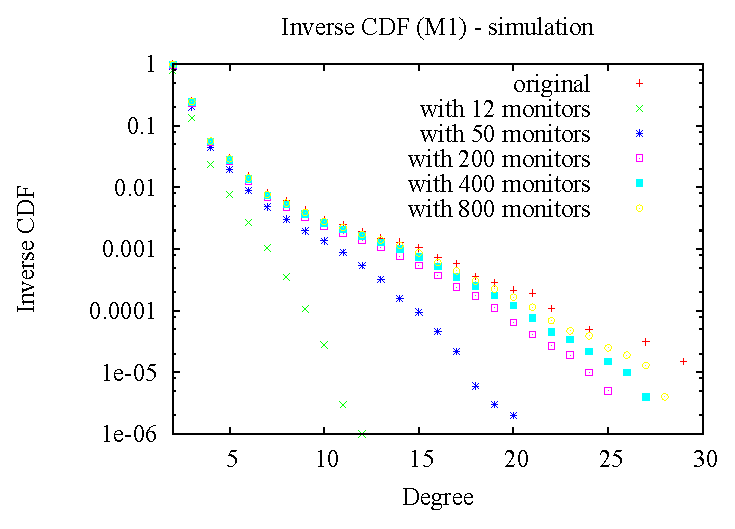
\includegraphics[width=0.9\columnwidth]{images/udpping-validation-simuls-icdf.eps}}\\
\subfloat{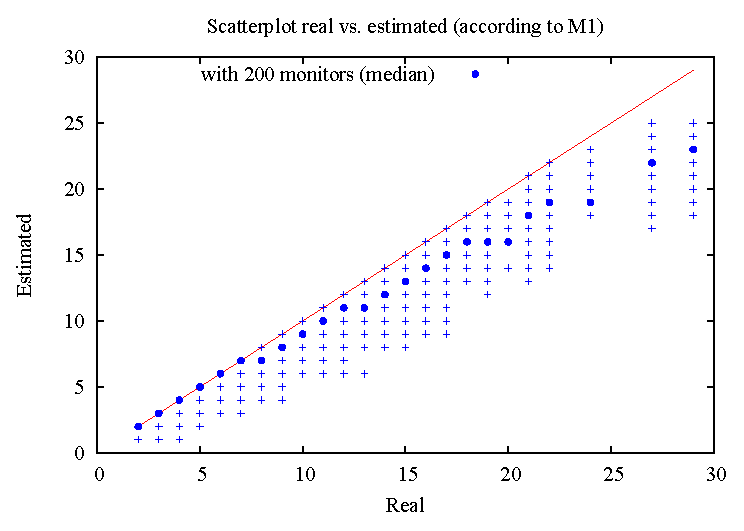
\includegraphics[width=0.9\columnwidth]{images/udpping-validation-simuls-correl.eps}}
\caption[Distributions observées dans les simulations de validation]{En haut, la
distribution de degrés observée pour différents nombre de moniteurs (qui
représentent ici des classes de colocalisation). En bas, la correlation entre le
degré observé par 200 moniteurs et le degré réel (un point par n\oe{}ud et
médiane).}
\label{fig:udpping-validation-simuls}
\end{figure}

Les résultats de ces simulations sont illustrés
en~\reffig{udpping-validation-simuls} (en haut), et sont constitués des
différentes distributions de degrés observées par les différents ensembles de moniteurs. On
constate que 200 moniteurs suffisent pour très bien observer la distribution de
degrés réelle, même si les fractions observée des n\oe{}uds des degrés élevés sont
moins bien estimées. La courbe met en évidence à quel point la proportion des
n\oe{}uds de faible degré est bien estimée : environ 95\% des n\oe{}uds de degré
inférieur ou égal à 10 sont bien observés avec leur degré réel avec 200
moniteurs.

Nous approfondissons en étudiant la différence absolue entre le degré observé
de chaque n\oe{}ud et son degré réel (\reffig{udpping-validation-simuls}, en
bas).
Cette approche confirme que notre méthode parvient très bien à mesurer le degré d'un n\oe{}ud en particulier --- ce qui est plus précis que de
correctement estimer la {\em distribution} des degrés. En particulier, la valeur médiane est
très proche du degré réel, même pour les n\oe{}uds de fort degré. Et même pour les
n\oe{}uds de degré élevé, la pire estimation, c'est à dire celle dont le degré
observé est le plus bas (donc le plus éloigné du degré réel) n'est jamais trop
éloignée du degré réelle. Par exemple, les n\oe{}uds de degré 29 ont dans le pire
cas été estimés comme ayant un degré de 18; les n\oe{}uds de degré 27 comme ayant
un degré de 17; et les n\oe{}uds de degré 24 comme ayant un degré de 18. Dans tous
les cas, comme nous l'avons déjà mentionné, un n\oe{}ud de fort degré n'est {\em
jamais} estimé comme ayant un {\em faible} degré; même dans le pire cas, il est
sous-évalué avec un facteur qui nous paraît raisonnable.

Nous pouvons conclure que les simulations sont en accord avec notre mesure
empirique. La distribution de degrés globale est très bien estimée (c'est à
dire que la distribution observée est très proche de la distribution réelle); en
particulier, la fraction des n\oe{}uds de faible degré est très précisément connue;
et en particulier, le degré de {\em chaque} n\oe{}ud est très bien estimé, pour peu
que son degré ne soit pas trop élevé. Augmenter le nombre de moniteurs (non
colocalisés) améliorerait la qualité de notre estimation, mais ne changerait pas
fondamentalement son aspect général.

\section{Discussion et conclusion}
\label{sec:udpping-conclusion}

Notre travail de mesure orientée propriété de la topologie physique d'Internet
nous a permis de mettre au point une méthode qui permet d'estimer la
distribution des degrés dans le c\oe{}ur de cette topologie. Cette estimation
peut être conduite depuis un ensemble relativement limité de moniteurs, et elle
est très fiable, à la fois dans sa forme générale, et dans la valeur précise des
fractions des n\oe{}uds de faible degré, sans commune mesure avec les
estimations tirées des cartes. Pour atteindre cet objectif, nous avons choisi de
définir très précisément notre objet d'étude et la propriété à laquelle nous
nous intéressions. En analysant les configurations qui pouvaient présenter des
problèmes, et en opérant un filtrage très prudent, nous assurons que les
résultats obtenus sont très fiables. Notre mesure réelle montre qu'en dépit de
ces filtrages très radicaux, nous arrivons à conserver suffisamment de données,
dont la fiabilité est garantie, pour réaliser une estimation statistiquement
pertinente. De plus, la précision de cette estimation peut encore être améliorée
en raffinant les conditions de la mesure, par exemple en itérant les mesures, en
augmentant le nombre de cibles, ou en augmentant le nombre de sites (classes de
colocalisation) depuis lesquels nous l'opérons. Nous avons utilisé les sites de
\planetlab, mais d'autres infrastructures, qui pourraient être utilisées en
complément de celle-ci, existent. \dimes~\cite{dimes} et
\ripeatlas~\cite{ripeatlas}, par exemple, mettent à disposition des milliers
d'hôtes pour des travaux de ce type. Depuis un tel ensemble de moniteurs et en
prenant les précautions nécessaires pour éviter d'encombrer le réseau, il n'est
pas exclu d'effectuer une mesure de très grande ampleur qui ciblerait {\em tout}
l'espace IPv4. En effet, même si notre approche distribuée peut sembler massive,
elle limite en réalité la charge induite sur les cibles au maximum à une sonde
envoyée par moniteur et par cible, en utilisant le protocole \udp qui est
rarement filtré sur le chemin puisqu'il est semblable à du trafic applicatif
normal. Cette faible charge se démarque des approches traditionelles basées sur
des outils comme \traceroute qui utilisent un très grand nombre de sondes.
Cette caractéristique de notre mesure nous permet d'ailleurs d'envisager une
utilisation de notre protocole sur la durée, en répétant notre mesure de manière
régulière au fil du temps, par exemple une fois par jour, afin de capturer la
dynamique de la topologie du c\oe{}ur.

Plutôt que de se hasarder à des hypothèses optimistes sur la bonne
implémentation des protocoles ou sur les bonnes pratiques du réseau, nous avons
volontairement limité la portée de nos résultats aux objets sur lesquels nous
pouvions présenter des garanties de fiabilité. Une conséquence de ce choix est
que la distribution de degrés que nous obtenons n'est pas la distribution de
degré de l'ensemble du la topologie physique, mais seulement du sous-graphe
constitué du c\oe{}ur d'Internet et de ses arêtes internes (les interfaces dans
le c\oe{}ur). Ce n'est pas forcément un problème, puisqu'il s'agit
précisément de la partie de la topologie dans laquelle opère le routage non
trivial. Hors du c\oe{}ur, le routage est le plus souvent limité à de
l'acheminement descendant ou ascendant dans des arbres ou des structures
arborescentes. Pour les travaux d'analyse du routage d'Internet, la
connaissance de la topologie du c\oe{}ur est donc bien souvent l'objet d'intérêt.
Pour autant, pour obtenir une connaissance complète de la distribution de degrés
de l'ensemble de la topologie physique, il faudrait certainement utiliser une
approche complémentaire, orthogonale à notre approche, pour obtenir une
connaissance spécifique du bord du réseau.

Au delà de la qualité de l'ensemble des moniteurs, il subsiste toutefois des
problèmes pratiques et conceptuels dans notre méthode. Le premier est, comme
nous l'avons déjà mentionné, sa précision limitée pour déterminer la fraction
des n\oe{}uds d'un degré élevé donné. En effet, même si nous pouvons avec précision
{\em majorer} la fraction des n\oe{}uds d'un degré {\em supérieur} à un degré
donné, notre méthode est intrinsèquement moins précise sur les degrés élevés,
dans la mesure où la probabilité d'observer une interface donnée d'un routeur
est \apriori plus faible si ce routeur est de degré élevé et qu'il faudra donc
un ensemble de moniteurs de meilleure qualité (en taille et en répartition) pour
la détecter. C'est d'autant plus vrai si l'utilisation de ses interfaces par un
routeur de fort degré n'est pas uniforme : si certaines interfaces du c\oe{}ur d'un
routeur sont très peu utilisées par rapport à d'autres, alors il sera plus
difficile de disposer d'un moniteur qui sollicite cette interface. La question
du choix de l'interface de réponse d'une cible en fonction du moniteur qui a
envoyé la sonde est d'ailleurs l'une de nos pistes de travail qui nous a semblé
les plus prometteuses et les plus pertinentes à l'issue de cette analyse, et
elle est le sujet d'intérêt du~\refchap{revtables}.


